\chapter{不等式和解不等式}

\section{大小次序与不等式}

\subsection{大小关系与次序关系}

“数系”的概念由于对于各种“量”的问题作了系统的讨论
而产生.由于计算个数和度量各种量的需要而产生了整数系
和实数系.日常生活的量与量的问题除了可以运算之外,还常
有很自然的“大小”关系,将这些关系抽象化,即得数与数之
间的大小关系,运算与大小关系是数系的两种基本结构.本章
将以数系在大小关系上的基本性质为出发点,逐步讨论不等
式的性质.

在日常生活中,我们说$A$量大于$B$量的意义是:“从$A$量
减去$B$量后还有剩余”,所以在数系中我们定义“$a$大于$b$”的意
义为$a-b$是一个正数.也就是:

\begin{blk}{定义}
\[\begin{split}
    a-b\text{是一个正数}&\Longleftrightarrow a>b\\
    a-b=0  &\Longleftrightarrow a=b\\
    a-b\text{是一个负数}&\Longleftrightarrow a<b
\end{split}\]
所以,$a>b$与$b<a$是同一回事.
\end{blk}


由这个定义,我们有下面的特例:
\[\begin{split}
    a>0 &\Longleftrightarrow a\text{是一个正数}\\
    a<0&\Longleftrightarrow a\text{是一个负数} 
\end{split}\]
这种正负数的表示法,前面已经用过.

我们知道任何一个实数或为正,或为零,或为负,上述
三种关系有且仅有一种成立.于是任意两个实数$a,b$的差$a-
b$也就或为正,或为零,或为负有且仅有一种成立.这也就是
说对于任意两个实数,我们都能比较它们的大小,下列关系
有一种且仅有一种成立:
\[a>b,\quad \text{或}\quad a=b,\quad  \text{或}\quad a<b\]

实数系的大小关系和直线上的点的次序关系具有相同的
构造,即坐标的大小关系就相当于相应点在数轴上的左右关
系.

我们可以这么来比着看:
\begin{enumerate}
    \item 0这个数把实数集$\mathbb{R}$分成三部分:$\mathbb{R}_+$, $\{0\}$,$\mathbb{R}_-$,
原点$O$这个点把数轴$\ell$分成三段:不含原点的正向射线$\ell_+$,原
点和不含原点的负向射线$\ell_-$;
\item 在数轴上任给两个点$A,B$, 我们在第二章1.2中已
经知道有向线段$\Vec{AB}$的数量
\[AB=x_B-x_A\]
这里$x_A,x_B$分别为$A,B$的坐标,于是
\[\begin{split}
    \text{$B$点在$A$点之右}&\Longleftrightarrow AB=x_B-x_A>0\Longleftrightarrow x_B>x_A\\
    \text{$B$点与$A$点重合}&\Longleftrightarrow AB=x_B-x_A=0\Longleftrightarrow x_B=x_A\\
    \text{$B$点在$A$点之左}&\Longleftrightarrow AB=x_B-x_A<0\Longleftrightarrow x_B<x_A\\
\end{split}\]
\end{enumerate}

基于上述实数的大小关系和数轴上点的次序关系之间的密切
对应,一切实数按照由小而大的顺序从左往右排列在数轴
上,这就使得我们可以由坐标的大小来确定直线上点的次序,
反过来,也用数轴上的点的次序来把数的大小关系形象化.

两个数或两个代数式用不等号“$>$”或“$<$”联结起来,以
表示它们的数量关系就构成不等式.

例如$5>3$, $-7<-4$, $x+1>3$, $a>b$等都是不等式.如
果不等式中含有变数,那么使不等式成立的变数值叫做不等
式的解,例如$x=2.1$是不等式$x+1>3$的一个解.使不等式成
立的变数值的全体,称为这个不等式的解集.一般来说,不等
式的解集是实数集的子集.例如不等式$x+1>3$的解集是:
$\{x|x\in\mathbb{R},\;\;x>2\}$.如果不等式的解集是全体实数集$\mathbb{R}$的话,
那么这种不等式称为恒不等式.例如$x^2+1>0$, 就是一个恒
不等式,如果不等式的解集是空集$\emptyset$的话,那么这种不等式是
不成立的或者说是矛盾的不等式,例如$x-1>x+1$, 就是
矛盾的不等式,由上面所说可以明白:一个含有变数的不等
式,只有在它的解集上才是成立的,譬如我们说$x+1>3$,
它只在$x>2$的条件下才是正确的.

有时我们会遇到用不等号“$\ge$”或“$\le$”联结的不等式,例
如$|x|\ge 2$, 其中“$\ge$”表示“$>$或$=$”,即其解集是
$$\{x|x\in\mathbb{R},\;\;|x|>2\}\cup\{x|x\in\mathbb{R},\;\;|x|=2\}$$
也就是$$\{x|x\in\mathbb{R},\;\;x\ge2\}\cup
\{x|x\in\mathbb{R},x\le -2\}$$
同样地“$\le$”表示“$<$或$=$”.我们也常写
$a<b<c$来表示$a<b$和$b<c$; $a<b\le c$表示$a<b$和$b\le c$.

我们可以把不等式解集用数轴或平面上的对应点集直观
地表示出来,如:
不等式$x+1>3$的解集可用图3.1表示,解点集是一条以
坐标是2的点为端点的开射线,由于2不包括在内,故用空
圈表示.

\begin{figure}[htp]
    \centering
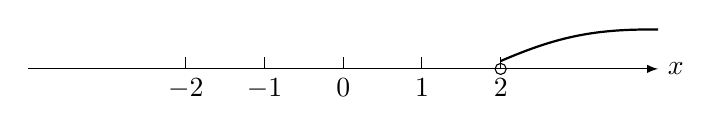
\begin{tikzpicture}[>=latex]
    \draw[->] (-4,0)--(4,0)node [right]{$x$};

\foreach \x in {-2,-1,...,2}
{
    \draw (\x,.15)--(\x, 0)node[below]{$\x$};
}
\draw (2,0) circle (2pt);

\draw[thick]  (2,0.1) to [bend left=12] (4,.5);


\end{tikzpicture}
    \caption{}
\end{figure}

不等式$|x|\ge 2$的解集可用图3.2表示,解集是两条射
线,一条是以坐标是2的点为端点的正向射线;另一条是以
坐标是$-2$的点为端点的负向射线.注意$\pm 2$处用实圈表示,
说明这两个点被包括在解集内.
\begin{figure}[htp]
    \centering
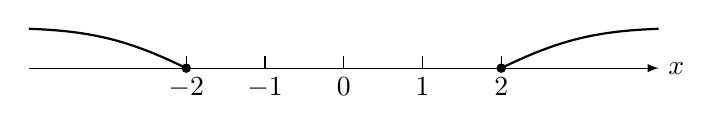
\begin{tikzpicture}[>=latex]
    \draw[->] (-4,0)--(4,0)node [right]{$x$};

\foreach \x in {-2,-1,...,2}
{
    \draw (\x,.15)--(\x, 0)node[below]{$\x$};
}
\draw (2,0)[fill=black] circle (1.5pt);  \draw (-2,0)[fill=black]  circle (1.5pt);

\draw[thick] (2,0) to [bend left=12] (4,.5);
\draw[thick]  (-2,0) to [bend right=12] (-4,.5);

\end{tikzpicture}
    \caption{}
\end{figure}


不等式$|x|\le 2$的解集可用图3.3表示,解点集是以$\pm 2$
为坐标的点为端点的线段.
\begin{figure}[htp]
    \centering
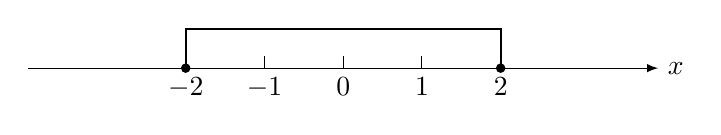
\begin{tikzpicture}[>=latex]
    \draw[->] (-4,0)--(4,0)node [right]{$x$};

\foreach \x in {-2,-1,...,2}
{
    \draw (\x,.15)--(\x, 0)node[below]{$\x$};
}
\draw (2,0)[fill=black] circle (1.5pt);  \draw (-2,0)[fill=black]  circle (1.5pt);

\draw[thick]  (-2,0)--(-2,.5)--(2,.5)--(2,0);

\end{tikzpicture}
    \caption{}
\end{figure}

学会不等式的解集合的图示,对以后解不等式是会有很
大好处的.

\begin{ex}
    \begin{enumerate}
    \item 在一条数轴上已知点$B$在$A,C$之间,如何用对应的数的
    大小来表示这种点的次序关系?
    \item 什么叫不等式、恒不等式、不等式的解?
    \item 试画出下列不等式解集图示:
    \begin{enumerate}
        \item $\{x|x\in\mathbb{R},\;\;x\ge -2\}$
        \item $\{x|x\in\mathbb{R},\;\;-1<x\le 3\}$
        \item $\{x|x\in\mathbb{R},\;\;x\ge 3\}\cup\{x|x\in\mathbb{R},\;\; x<-1\}$
        \item $\{x|x\in\mathbb{R},\;\;x\le 2\}\cap \{x|x\in\mathbb{R},\;\; x\le 3\}$
    \end{enumerate}
    
\end{enumerate}
\end{ex}

\subsection{不等式的基本性质}
基于实数系中大于和小于的定义以及实数系中的下列性
质,即
\begin{blk}{}
\begin{enumerate}
    \item 正数加正数仍是正数;
    \item 正数乘正数仍是正数;
    \item 正数乘负数则为负数;
    \item 负数乘负数则为正数;
    \item 任何一数或为正,或为零,或为负,且这三种可能
性有一种且仅有一种成立.
\end{enumerate}
\end{blk}

我们说明不等式的基本性质如下:
\begin{blk}{性质1}
    如果$a>b$, $b>c$, 那么$a>c$ (不等式传递性).
\end{blk}

\begin{proof}
    $a>b$, $b>c$就是$a-b>0$, $b-c>0$.
由于
$$a-c=(a-b)+(b-c)>0$$
这就是说:
$a>c$    
\end{proof}

\begin{blk}{性质2}
    如果$a>b$, 那么对于任意的$c$, 有$a+c>b+c$
(两边同加一个数,不等号方向不变).
\end{blk}

\begin{proof}
    $a>b$,就是$a-b>0$,
    由于
    $$(a+c)-(b+c)=a-b$$
    所以
    $$(a+c)-(b+c)>0$$
    这就是:
$a+c>b+c$
\end{proof}

\begin{blk}{推论1}
不等式中任何一项可以把它的符号变成相反的
符号后,从一边移到另一边.

\end{blk}

\begin{blk}{推论2}
    如果$a>b$, $c>d$, 那么$a+c>b+d$ (同向不等式的两端相加仍得同向不等式).
    \end{blk}

这是因为,根据性质2, 可得$a+c>b+c$,$b+c>b+
d$再根据性质1,可得$a+c>b+d$.

\begin{blk}{性质3}
如果$a>b$,$c>0$,那么$ac>bc$,如果$c<0$,
那么$ac<bc$,(不等式两端乘以正数得同向不等式,乘以负
数得反向不等式).
\end{blk}

\begin{proof}
$a>b$就是$a-b>0$,
由于
$$ac-bc=(a-b)c$$
所以当$c>0$时,$ac-bc>0$, 就是说
$$ac>bc$$
当$c<0$时,$ac-bc<0$, 就是说
$$ac<bc$$
\end{proof}

\begin{blk}{推论1}
   $a>b$和$b<a$是等价的,即:如果$a>b$,那么
$b<a$;反过来,如果$b<a$,那么$a>b$.
\end{blk}

这是因为$a>b$就是$a-b>0$, 不等式两边乘以$-1$, 得
$-(a-b)<0$, 即$b-a<0$, 这就是$b<a$, 同理可证后半个
结论.

\begin{blk}{推论2}
    如果$a>b>0$, $c>a>0$, 那么$ac>bd$.
\end{blk}

 
这是因为$a>b$, $c>0$, 根据性质3, 可得:
\begin{equation}
    ac>bc
\end{equation}
又$c>d$, $b>0$, 同理得
\begin{equation}
    bc>bd
\end{equation}
由(3.1),(3.2)得:
\begin{equation*}
    ac>bd  \tag{性质1}
\end{equation*}

\begin{blk}{推论3}
    如果$a>b$, 并且$a,b$同号,那么$\frac{1}{a}<\frac{1}{b}$
\end{blk}

因为$\frac{1}{b}-\frac{1}{a}=\frac{a-b}{ab}$,再由假设得到:
\[a-b>0,\quad ab>0\]
所以$\frac{1}{b}-\frac{1}{a}>0$,即$\frac{1}{a}<\frac{1}{b}$.

\begin{blk}{推论4}
    如果$a>b>0$, 那么$a^n>b^n$ ($n$是大于1的整
数).
\end{blk}

\begin{itemize}
    \item 当$n=2$时,由$a>b>0$,根据推论2得到:
$a^2>b^2$
\item 当$n=3$时,由$a>b>0$和$a^2>b^2$, 同理得到:
$a^3>b^3$
\item 依此类推,得到:$a^n>b^n$
\end{itemize}
这样正数之间的不等式可以进行$n$次乘方运算,仍得同向不
等式.

\begin{blk}{推论5}
    如果$a>b>0$, 那么$\sqrt[n]{a}>\sqrt[n]{b}$ ($n$是大于1的整
数).
\end{blk}

因为$\sqrt[n]{a}$, $\sqrt[n]{b}$是$n$次算术根,所以它们都是正数.

假设$a^{\tfrac{1}{n}}=b^{\tfrac{1}{n}}$,于是$\left(a^{\tfrac{1}{n}}\right)^n=\left(b^{\tfrac{1}{n}}\right)^n$,因而$a=b$,这就与已知$a>b$矛盾.

假设$a^{\tfrac{1}{n}}<b^{\tfrac{1}{n}}$,于是$\left(a^{\tfrac{1}{n}}\right)^n<\left(b^{\tfrac{1}{n}}\right)^n$,即$a<b$,这又与
已知条件矛盾.但是$\sqrt[n]{a}$和$\sqrt[n]{b}$的大小关系,只有三种可能,
而且仅有一种成立,因此$\sqrt[n]{a}>\sqrt[n]{b}$.
这样正数之间的不等式可以进行开$n$次方运算,仍得同向不
等式.

下面我们从不等式的定义和不等式的基本性质及其推论
出发来证明一些恒不等式.在推导不等式时,我们常利用实
数的平方不会是负的这个事实.我们首先证明下面的命题:

\begin{blk}{命题}
    若$a$是任意实数,那么$a^2\ge 0$.
\end{blk}

事实上,$a$或是正数,或是零,或是负数.如果$a>0$,
那么$a^2=a\x a>0$; 如果$a=0$, 那么$a^2=0\x0=0$; 如果
$a<0$, 于是$a=-|a|$, $a^2=(-|a|)\cdot (-|a|)=|a|^2>0$, 无
论哪种情形都有$a^2\ge 0$.

\subsubsection{比较法}

为证明某一个不等式成立,常用“大于”
定义,即要证$a>b$, 我们常证$a-b>0$, 这种方法叫做比较
法.用比较法证明不等式时,常常要把式子配方或把式子分
解成恒取正值或负值的因式的乘积.

\begin{example}
    若$a,b$是实数,则
    \begin{equation}
        a^2+b^2\ge 2ab
    \end{equation}
\end{example}
\begin{proof}
    $\because\quad a^2+b^2-2ab=(a-b)^2\ge 0$

    $\therefore\quad a^2+b^2\ge 2ab$,当且仅当$a=b$时,取等号.
\end{proof}

    
\begin{example}
    若$a,b,c$是任何实数,求证:
    \begin{equation}
   a^2+b^2+c^2\ge ab+bc+ca     
    \end{equation}
\end{example}

\begin{proof}
    \[\begin{split}
     &\quad   a^2+b^2+c^2-ab-bc-ca \\
      &=\frac{1}{2}( 2a^2+2b^2+2c^2-2ab-2bc-2ca)\\
        &=\frac{1}{2}\left[(a^2-2ab+b^2)+(b^2-2bc+c^2)+(c^2-2ca+a^2)\right]\\
        &=\frac{1}{2}\left[(a-b)^2+(b-c)^2+(c-a)^2\right]\ge 0
    \end{split}\]
   
    这里等于关系成立等同于$(a-b)^2=(b-c)^2=(c-a)^2=0$.
    即$a=b=c$, 因此,
$a^2+b^2+c^2\ge ab+bc+ca $
这里当且仅当$a=b=c$时取等号.

\textbf{另证:} 
\[\begin{split}
    &\quad   a^2+b^2+c^2-ab-bc-ca \\
&=a^2-(b+c)a+b^2+c^2-bc\\
&=\left[a^2-(b+c)a+\left(\frac{b+c}{2}\right)^2\right]+b^2+c^2-bc-\frac{(b+c)^2}{4}\\
&=\left(a-\frac{b+c}{2}\right)^2+\frac{3}{4}(b-c)^2\ge 0
\end{split}\]

这里等于关系当且仅当$b=c$和$a=\frac{b+c}{2}$
时,即$a=b=c$时成
立,因此,
$a^2+b^2+c^2\ge ab+bc+ca $.
\end{proof}




\begin{example}
    若$a,b$是不相等的正数,则
\[\frac{a}{\sqrt{b}}+\frac{b}{\sqrt{a}}>\sqrt{a}+\sqrt{b}\]
\end{example}
    
\begin{proof}
\[\begin{split}
     \frac{a}{\sqrt{b}}+\frac{b}{\sqrt{a}}-\sqrt{a}-\sqrt{b}
    &=\frac{a\sqrt{a}+b\sqrt{b}-a\sqrt{b}-b\sqrt{a}}{\sqrt{ab}}\\
    &=\frac{a\left(\sqrt{a}-\sqrt{b}\right)-b\left(\sqrt{a}-\sqrt{b}\right)}{\sqrt{ab}}\\
    &=\frac{\left(\sqrt{a}-\sqrt{b}\right)(a-b)}{\sqrt{ab}}\\
    &=\frac{\left(\sqrt{a}-\sqrt{b}\right)^2\left(\sqrt{a}+\sqrt{b}\right)}{\sqrt{ab}}>0
\end{split}\]

因为算术根式$\sqrt{ab}$, $\sqrt{a}+\sqrt{b}$在$a,b$是正数的条件
下是正数,又$a\ne b$,因此$\left(\sqrt{a}-\sqrt{b}\right)^2>0$.

所以,$\frac{a}{\sqrt{b}}+\frac{b}{\sqrt{a}}>\sqrt{a}+\sqrt{b}$
\end{proof}

\subsubsection{综合法}
要证明某个不等式,常由已知的或明显
的不等式,根据不等式的性质把它推导出来,这种由因导果
的证法叫做综合证法.
\begin{example}
    如果$a>b>0$, $0<c<d$,那么
    \begin{equation}
        \frac{a}{c}>\frac{b}{d}
    \end{equation}
\end{example}

\begin{proof}
 因为$c,d$同为正数,又$c<d$, 根据性质3的推
论3,得\[\frac{1}{c}>\frac{1}{d}>0\]
又$a>b>0$,
根据性质3的推论2, 得   
\[\frac{a}{c}>\frac{b}{d}\]
\end{proof}
    
\begin{example}
    $a_1$, $a_2$是任意正数,试证:
\begin{equation}
    \frac{a_1+a_2}{2}\ge \sqrt{a_1a_2}
\end{equation}
这里当且仅当$a_1=a_2$时,取“$=$”号.
\end{example}

\begin{proof}
    因为$(a_1-a_2)^2\ge 0$, 由此得到
\[a_1^2-2a_1a_2+a_2^2\ge 0\]
移项:
\[a^2_1+a^2_2\ge 2a_1a_2\]
两边同加正数$2a_1a_2$, 得
\[\begin{split}
    a_1^2+2a_1a_2+a^2_2&\ge 4a_1a_2\\
(a_1+a_2)^2&\ge 4a_1a_2
\end{split}\]

根据性质3的推论5, 得
\[a_1+a_2\ge 2\sqrt{a_1a_2}\]
即:$\frac{a_1+a_2}{2}\ge \sqrt{a_1a_2}$

显然,当且仅当$a_1=a_2$时,不等式取等号.
\end{proof}

这个不等式很重要,我们叫
$\frac{a_1+a_2}{2}$为正数$a_1$, $a_2$的算术
平均值,叫$\sqrt{a_1a_2}$为正数$a_1$, $a_2$的几何平均值.上面的不等
式是说两个正数的算术平均值不小于它们的几何平均值.

这个不等式有下面的几何
意义:

\begin{figure}[htp]
    \centering
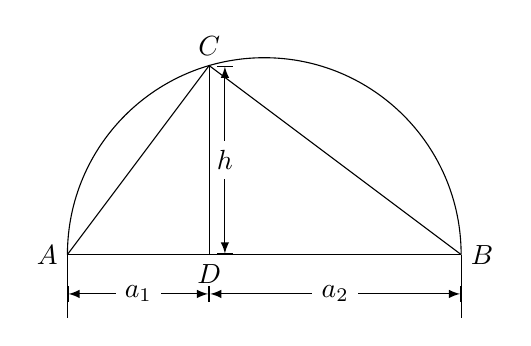
\begin{tikzpicture}[>=latex]
    \draw[|<->|] (2,0)--node[fill=white]{$h$}(2,2.4);
 \draw (0,0)node[left]{$A$}--(5,0)node[right]{$B$};
\draw (5,0) arc (0:180:2.5);    
\draw (1.8,2.4)node[above]{$C$}--(1.8,0)node[below]{$D$};
\draw (0,0)--(1.8,2.4)--(5,0);
\draw[|<->|] (0,-.5)--node[fill=white]{$a_1$}(1.8,-.5);
\draw[|<->|] (5,-.5)--node[fill=white]{$a_2$}(1.8,-.5);
\draw (0,0)--(0,-.8);\draw (5,0)--(5,-.8);

\end{tikzpicture} 
    \caption{}
\end{figure}


以$a_1+a_2$为半径作圆
(图3.4), 设$AD=a_1$, $DB=a_2$,
过$D$点作线段$AB$的垂直线交
半圆于$C$点,于是$\angle ACB=
90^{\circ}$, 设$DC=h$, 由勾股定理
知:
\[AD^2+DC^2=AC^2,\qquad DC^2+DB^2=BC^2,\qquad AC^2+BC^2=AB^2\]
即:
$(a_1^2+h^2)+(a_2^2+h^2) =(a_1+a_2)^2$
从而:
\[h=\sqrt{a_1a_2}\]

另一方面,$DC$无论如何是不会超过圆的半径的,即:
\[h=\sqrt{a_1a_2}\le \frac{a_1+a_2}{2}\]
此外,当且仅当$D$点与圆心$O$点重合时,即$a_1=a_2$时,$DC$等
于圆的半径,即$h=\sqrt{a_1a_2}=\frac{a_1+a_2}{2}$    

\begin{example}
    两个正数的和是定值$A$, 求证在所有这样的和
中,当且仅当这两数相等时,它们的乘积最大.
\end{example}

\begin{proof}
设两个正数是$x$和$y$, 由题设知
\begin{equation}
   x+y=A 
\end{equation}
而其积依例3.5应该适合不等式:
\[\sqrt{xy}\le \frac{x+y}{2}\]
也即:$xy\le \left(\frac{x+y}{2}\right)^2$
将条件(3.7)代入上面不等式中,得
\[xy\le \left(\frac{A}{2}\right)^2\]
这表示其和等于$A$的两个正数,无论怎样取法,它们的积都
不大于常数$\left(\frac{A}{2}\right)^2$.
由于这里等式当且仅当两个正数相等时,
即$x=y=\frac{A}{2}$时,才能成立,因此当且仅当两个正数相等时,
它们的积才能达到最大值$\left(\frac{A}{2}\right)^2$.

\end{proof}
    
\begin{example}
$a_1,a_2,a_3$为任意正数,求证:
\begin{equation}
 \frac{a_1+a_2+a_3}{3}\ge \sqrt[3]{a_1a_2a_3}  
\end{equation}
这里的等于关系当且仅当$a_1=a_2=a_3$时成立.
\end{example}

\begin{proof}
    如果令$b_1>0$, $b_2>0$, $b_3>0$, 使得
\[a_1=b_1^3,\qquad a_2=b_2^3,\qquad  a_3=b_3^3\]
这样一来,我们就要证明:
\[b_1^3+b_2^3+b_3^3\ge 3b_1b_2b_3\]
由于
$b_1^3+b_2^3=(b_1+b_2)(b_2^2-b_1b_2+b^2_2)$
利用不等式(3.3)或(3.6),就有:
\[b_1^2 -b_1b_2+b_2^2\ge b_1b_2\]
所以我们有:
\[b^3_1+b_2^3\ge b_1b_2(b_1+b_2)=b_1^2 b_2+b_1b_2^2\]
同样地可证明:
\[b_2^3+b_3^3\ge b_2^2b_3+b_2b^2_3\]
以及
\[b_3^3+b_1^3\ge b_3^2b_1+b_3b^2_1\]
从而
\[\begin{split}
    2(b_1^3+b_2^3+b_3^3) &\ge b_1(b^2_2+b^2_3)+b_2(b^2_3+b^2_1)+b_3(b^2_1+b^2_2)\\
    &\ge b_1(2b_1b_2)+b_2(2b_3b_1)+b_3(2b_1b_2)\\
    &=6b_1b_2b_3
\end{split}\]
即:$b_1^3+b_2^3+b_3^3\ge 3b_1b_2b_3$

因而,$\frac{a_1+a_2+a_3}{3}\ge \sqrt[3]{a_1a_2a_3}  $

此外,从上面的过程可见,等式成立,等同于要求
\[b_1^2-b_1b_2 +b_2^2=b_1b_2,\qquad  b_2^2 -b_2b_3+b_3^2 =b_2b_3,\qquad b_3^2-b_3b_1+b_1^2=b_2b_1\]
三个式子成立,这就等同于要求
$b_1=b_2=b_3$.
\end{proof}

\begin{rmk}
    如果我们注意下面的因式分解:
    \[b_1^3+b_2^3+b_3^3-3b_1b_2b_3=(b_1+b_2+b_3)(b_1^2+b_2^2
    +b^2_3-b_1b_2-b_2b_3-b_3b_1)\]
    那么,我们就立即可得不等式(3.8)的证明.但是这样的因式
    分解不易使人想到,而且也不能进一步推广. 
\end{rmk}

由不等式(3.6)和(3.8)使人猜想,对于$n$个正数:
$a_1,a_2,\ldots,a_n$是不是有:
\[\frac{a_1+a_2+\cdots+a_n}{n}\ge \sqrt[n]{a_1a_2\cdots a_n}\]
其中$n$是大于1的整数,当且仅当$a_1=a_2=\cdots=a_n$时取等号.

我们说这个一般的结论“$n$个正数的算术平均不小于几何
平均”是成立的,不过这里我们略去它的证明.

\begin{example}
    求证在周长都为$2L$的所有三角形中,面积最大
的必是等边三角形.
\end{example}

\begin{proof}
    设三角形边长为$a,b,c$, 则周长为$a+b+c=2L$,
设面积为$S$, 于是依不等式(3.8)
\[\begin{split}
    S^2&=L(L-a)(L-b)(L-c)\\
&\le L\left[\frac{(L-a)+(L-b)+(L-c)}{3}\right]^3\\
&=\frac{L^4}{27}
\end{split}\]

因此这样的三角形面积不会超过$\frac{L^2}{\sqrt{27}}$,
同时要达到这个数
值必须且只须$L-a=L-b=L-c$, 即为等边三角形.
\end{proof}
    
\begin{example}
    若$x,y,z$是不都相等的正数,且$x+y+z=1$

求证$(1-x)(1-y)(1-z)>8xyz$.
\end{example}

\begin{proof}
由于:
\[\begin{split}
    1-z&=x+y\ge 2\sqrt{xy}\\
1-y&=x+z\ge 2\sqrt{xz}\\
1-x&=y+z\ge 2\sqrt{yz}
\end{split}\]   
因为$x,y,z$不都相等,即至少有两个数不相等,所以上面
三个不等式中至少有一个不等式只能成立“$>$”关系,将上面
不等式的两端相乘得到
\[(1-x)(1-y)(1-z)>8\sqrt{x^2y^2z^2}=8xyz\]
\end{proof}

\subsubsection{分析法}
证明不等式也可以用分析法,就是先假
定这个不等式成立,逐步找出使这个不等式成立的充分条
件,直到推导出已知条件或明显的不等式为止.也就是说由
果索因找出证题路线,然后再按分析过程的相反过程写出由
已知条件导出结论的过程.应用分析法时,一定要仔细检查
每步推理是否可逆,也就是不等式在反推时有无不等式的性
质作根据,如果其中某一步推理不可逆,那么用分析法是无
效的.



\begin{example}
    试证$\left(\sqrt{2}+1\right)^2 <3.4\sqrt{3}$

\end{example}

\begin{proof}
要证
\begin{equation}
    \left(\sqrt{2}+1\right)^2 <3.4\sqrt{3}
\end{equation}
成立 即要证:$3+2\sqrt{2}<\frac{17}{5}\sqrt{3}$.

两边乘以5,只须证:
\begin{equation}
    15+10\sqrt{2}<17\sqrt{3}
\end{equation}
两边平方,可证:
\begin{equation}
    225+200+300\sqrt{2}<867
\end{equation}
移项
\begin{equation}
    300\sqrt{2}<442
\end{equation}
两边除以300,即要证:
\begin{equation}
    \sqrt{2}<1.47
\end{equation}
显然(3.13)成立,而由(3.9)推出(3.13)的每一步都可逆,
所以$\left(\sqrt{2}+1\right)^2 <3.4\sqrt{3}$成立.
\end{proof}
    
\begin{example}
    若$a>b>0$, 求证:
    \[\frac{1}{8}\frac{(a-b)^2}{a}<\frac{a+b}{2}-\sqrt{ab}<\frac{1}{8}\frac{(a-b)^2}{b} \]
\end{example}

\begin{proof}
    (分析法)要证:$\frac{a+b}{2}-\sqrt{ab}<\frac{1}{8}\frac{(a-b)^2}{b}$成立,只须证:
\[\frac{\left(\sqrt{a}-\sqrt{b}\right)^2}{2}<\frac{1}{8}\frac{(a-b)^2}{b}\]

$\because \quad a>b>0,\qquad \therefore\quad \left(\sqrt{a}-\sqrt{b}\right)^2\ne 0$,两边除以$\left(\sqrt{a}-\sqrt{b}\right)^2$,可证:
\[\frac{\left(\sqrt{a}+\sqrt{b}\right)^2}{8b}>\frac{1}{2}\]
但是,$\frac{\left(\sqrt{a}+\sqrt{b}\right)^2}{8b}=\frac{1}{8}\left(1+\sqrt{\frac{a}{b}}\right)^2$,即要证:
\[\frac{1}{8}\left(1+\sqrt{\frac{a}{b}}\right)^2>\frac{1}{2},\quad \text{或}\quad \left(1+\sqrt{\frac{a}{b}}\right)^2>4\]

两边开平方取算术根,可证:
\[1+\sqrt{\frac{a}{b}}>2,\quad \text{或}\quad \sqrt{\frac{a}{b}}>1\]
即要证:$a>b$.

但是,$a>b>0$成立,并且上面推理的每一步可逆,所以,
$\frac{a+b}{2}-\sqrt{ab}<\frac{1}{8}\frac{(a-b)^2}{b}$成立.

同理证明:$\frac{a+b}{2}-\sqrt{ab}>\frac{1}{8}\frac{(a-b)^2}{a}$成立.

因此,$\frac{1}{8}\frac{(a-b)^2}{a}<\frac{a+b}{2}-\sqrt{ab}<\frac{1}{8}\frac{(a-b)^2}{b}$
\end{proof}

\begin{rmk}
    此题分析中的关键:
    \begin{enumerate}
        \item 通过恒等变形,将不等
    式两边的正因式$\left(\sqrt{a}-\sqrt{b}\right)^2$约去;
    \item $\frac{\left(\sqrt{a}+\sqrt{b}\right)^2}{8b}=\frac{1}{8}\left(1+\sqrt{\frac{a}{b}}\right)^2$的右端使求证和已知条件的联系明朗化.
    \end{enumerate}
\end{rmk}



\begin{example}
    试证:若$a>0$, $b^2-4ac\le 0$, 则对于任意实数
\begin{equation}
    ax^2+bx+c\ge 0
\end{equation}
\end{example}

\begin{proof}
\[\begin{split}
    ax^2+bx+c&=a\left[x^2+\frac{b}{a}x+\left(\frac{b}{2a}\right)^2\right]+c-\frac{b^2}{4a}\\
    &=a\left(x+\frac{b}{2a}\right)^2+\frac{4ac-b^2}{4a}
\end{split}\]
因为不论$x$为何值,$\left(x+\frac{b}{2a}\right)^2\ge 0$, 又因为:
$b^2-4ac\le 0$,故$4ac-b^2\ge 0$,因而:
\[ax^2+bx+c=a\left(x+\frac{b}{2a}\right)^2+\frac{4ac-b^2}{4a}\]
的值的正、负与$a$的值的正、负相同,并且当且仅当$b^2-4ac=0$和$x=-\frac{b}{2a}$
时,其值为零,故在$a>0$, $b^2-4ac\le 0$的条件下,不论$x$为何值,
$ax^2+bx+c\ge 0$.
\end{proof}

\begin{rmk}
    二次三项式经过配方后,要解决的问题就明朗
    化了.    
\end{rmk}


\begin{example}
    试证:对于任意实数$a_1,a_2,a_3$; $b_1,b_2,b_3$, 有
  \begin{equation}
      (a_1^2+a_2^2+a_3^2)(b_1^2+b_2^2+b_3^2)\ge (a_1b_1+a_2b_2+a_3b_3)^2
  \end{equation} 
\end{example}

\begin{proof}
    \[\begin{split}
&\quad   (a_1^2+a_2^2+a_3^2)(b_1^2+b_2^2+b_3^2)-(a_1b_1+a_2b_2+a_3b_3)^2\\
 & = a_1^2b_1^2+a_1^2b_2^2+a_1^2b_3^2
    +a_2^2b_1^2+a_2^2b_2^2+a_2^2b_3^2
    +a_3^2b_1^2+a_3^2b_2^2+a_3^2b_3^2\\
  &\qquad  + a_1^2b_1^2-a_2^2b^2_2-a_3^2b_3^2
    -2a_1b_1a_2b_2-2a_1b_1a_3b_3-2a_2b_2a_3b_3\\
    & = (a_1^2b_2^2-2a_1b2b_2a_2b_1+a_2^2+a_2^2b_1^2)
    +(a_1^2b_3^2-2a_1b_3a_3b_1+a_3^2b_1^2)\\
    &\qquad     +(a_2^2b_3^2-2a_2b_3a_3b_2+a_3^2b_2^2)\\
    & = (a_1b_2 -a_2b_1)^2+(a_1b_3-a_3b_1)^2+(a_2b_3-a_3b_2)^2\\
    & \ge 0        
    \end{split}\]
    这里不等式当且仅当$a_1b_2 -a_2b_1=a_1b_3-a_3b_1=a_2b_3-a_3b_2=0$   
    时,即在$\frac{a_1}{b_1}=\frac{a_2}{b_2}=\frac{a_3}{b_3}$时取等号. 
\end{proof}

不等式(3.15)可以推广到下面的情形:

\begin{blk}{}
    对于$a_1,a_2,\ldots,a_n$; $b_1,b_2,\ldots,b_n$的一切实数值,下列
    不等式成立:
    \[(a_1b_1+a_2b_2+\cdots+a_nb_n)^2\le (a_1^2+a_2^2+\cdots+a_n^2)(b_1^2+b_2^2+\cdots+b_n^2)\]
    等式当且仅当
    $\frac{a_1}{b_1}=\frac{a_2}{b_2}=\cdots=\frac{a_n}{b_n}$
    时成立,这个不等式称为
    柯西不等式,不等式(3.15)是柯西不等式$n=3$的特例.
\end{blk}



\begin{example}
    试证:如果$a^2+b^2+c^2=1$和$x^2+y^2+z^2=1$, 这
里$a,b,c$不分别等于$x,y,z$,那么,
\[ax+by+cz<1\]
\end{example}

\begin{proof}
根据柯西不等式,有
\[(ax+by+cz)^2<(a^2+b^2+c^2)(x^2+y^2+z^2)\]
(因为$a,b,c$不分别等于$x,y,z$, 故不能取等号).由此
\[(ax+ay+cz)^2<1\]
即:$|ax+by+cz|<1$,但是
\[ax+by+cz\le |ax+by+cz|\]
所以:$ax+by+cz<1$
\end{proof}

\section*{习题3.1}
\addcontentsline{toc}{subsection}{习题3.1}
\begin{enumerate}
    \item 如果$a>b$, $e>f$, $c>0$, 求证$f-ac<e-bc$.
    \item 如果$a>b$, $g<0$, $c$是任何数,求证:
   \[ g(a-c)<g(b-c)\]

   \item   如果$a>b>0$, $c>d>0$, 求证
   $\frac{1}{ac}<\frac{1}{bd}$
   \item 如果$a>b>0$, $c<d<0$, $e<0$, 求证:
   $\frac{e}{a-c}>\frac{e}{b-d}$
   \item 如果$a,b$是正数,求证:
   \[\frac{a+b}{1+a+b}<\frac{a}{1+a}+\frac{b}{1+b}\]
   \item 回答下列问题,并说明理由(“是”的给予证明;“不是”
   的举一反例).
\begin{enumerate}
    \item 如果$a>b$, $c=d$是否一定有$ac>bd$?
    \item 如果$\frac{a}{c^2}<\frac{b}{c^2}$,
    是否一定有$a<b$?
    \item 如果$ac>bc$, 是否一定有$a>b$?
    \item 如果$a>b$, $c>d$, 是否一定有$a-c>b-d$?
    \item 如果$a>b>0$, $c>d>0$, 是否一定有$\frac{a}{c}>\frac{b}{d}$?
    \item 如果$a>b$, $c>d$, 是否一定有$ac>bd$?
    \item 如果$a>b$, 是否一定有$a^2>b^2$?
    \item 如果$a>b$, 是否一定有$a^3>b^3$?
\end{enumerate}

\textbf{用比较法证明下面不等式:}
\item 若$a,b$是正数,求证$\frac{a^2+b^2}{2}\ge \left(\frac{a+b}{2}\right)^2$
\item $1+2x^4\ge x^2+2x^3$
\item 若$a,b$是正数,求证$a^3+b^3\ge a^2b+ab^2$
\item 证明: $a^2+b^2+c^2\ge 2(a+b+c)-3$
\item 若$a,b,c$是正数,求证
$a^2(b+c) +a(b^2+c^2-bc)> 0$


\textbf{用综合法证明下面不等式:}
\item 证明$\frac{a}{b}+\frac{b}{a}\ge 2$, 其中$a,b$是正数.
\item 若$a,b,c$是正数,求证:
\[\frac{ab(a+b)+ac(a+c)+bc(b+c)}{abc}\ge 6\]


\item 设$a,b$是不相等的正数,求证:
\begin{enumerate}
    \item $(a+b)(a^2+b^2)(a^3+b^3)>8a^3b^3$
    \item $(a+b)(a^3+b^3)>(a^2+b^2)$
\end{enumerate}

\item 若$a_1,a_2,a_3,a_4$都是正数,求证:
\[\frac{a_1+a_2+a_3+a_4}{4}\ge \sqrt[4]{a_1a_2a_3a_4}\]
\item 在上题中,令$a_4=\frac{a_1+a_2+a_3}{3}$,
试由\[\left(\frac{a_1+a_2+a_3+a_4}{4}\right)^4\ge a_1a_2a_3a_4\]
推出$\frac{a_1+a_2+a_3}{3}\ge \sqrt[3]{a_1a_2a_3}$

\item 若$a,b,c$是正数,求证:
$a+b+c\ge \sqrt{ab}+\sqrt{bc}+\sqrt{ca}$
\item 若$a,b$是正数,求证:
$\frac{a^3+b^3}{2}\ge \left(\frac{a+b}{2}\right)^3$
\item 若$a,b,c$是不相等的正数,
求证$(a+b+c)\left(\frac{1}{a}+\frac{1}{b}+\frac{1}{c}\right)>9$

\item 若$x>0$, 求证$x+\frac{9}{x}$
的最小值是6.
\item 当$x$为何值时,$2x(9-2x),\quad \left(0<x<\frac{9}{2}\right)$
取最大值,
最大值是多少?
\item 求证:周长一定的所有矩形中以正方形的面积最
大;面积一定的所有矩形中以正方形的周长最短,
这个正方形的边长是多少?
\item  斜边长一定的直角三角形中,求两直角边的和的最大
值,又何时达到最大值.


\textbf{用综合法或分析法证明下面不等式:}

\item 求证:
\begin{multicols}{2}
\begin{enumerate}
    \item $\sqrt{2}+\sqrt{3}<4$
    \item $\sqrt{3}+\sqrt{5}>\sqrt{15}$
    \item $\sqrt{2}+\sqrt{3}<\sqrt{10}$
    \item $\sqrt{5}+\sqrt{7}>1+\sqrt{15}$
\end{enumerate}    
\end{multicols}

\item 下面的差是正的还是负的?
\[\sqrt[3]{3}-\sqrt{2},\qquad \sqrt[4]{3}-\sqrt[5]{4},\qquad \sqrt[5]{2}-\sqrt[6]{3} \]
\item 若$a,b,c$是正整数,求证:
$ab+bc+ac\le 3abc$

\item 求证$a_1+a_2+\cdots+a_n<\frac{1}{1-a}\quad (0<a<1)$

\item 若$|a|<1$, $|b|<1$, 求证:$\left|\frac{a+b}{1+ab}\right|<1$

\item 求证$\frac{x^2+2}{\sqrt{x^2+1}}\ge 2$

\item 若$a,b,c,d$是正数,求证:
$$\sqrt{(a+c)(b+d)}\ge \sqrt{ab}+\sqrt{cd}$$
\item 若$a>b>0$且$m>n$, 求证:
$\frac{a-b}{a^m+b}>\frac{a-b}{a^n+b}$

\item 若$a>0$, $b>0$且$a+b=1$, 求证:
$\left(a+\frac{1}{a}\right)\left(b+\frac{1}{b}\right)\ge \frac{25}{4}$
\end{enumerate}

\section{解不等式}
解不等式就是要找出使不等式成立的变数值的全体,即
不等式的解集,在上节1.1中我们已经知道含有一个变数的
不等式的解集,或是整个实数集$\mathbb{R}$, 或是实数集$\mathbb{R}$的一个子
集,或是空集$\emptyset$.

解不等式的方法如同解方程一样,在于应用不等式的性
质,逐步将它变形到最简单的不等式,在变形过程中要特别注
意合理地应用不等式的性质,以保证每次得到的不等式的解
集和原来的不等式的解集都相同.现在让我们分析一下怎样
的变形可以保证解集相同,设不等式$\alpha(x)>0$和$\beta(x)>0$的对
应解集是$A$和$B$, 这里$\alpha(x)$, $\beta(x)$代表含有一个变数的代数式.

假设任意给出$x\in A$使$\alpha(x)>0$成立,根据不等式的性质
作变形推出$\beta(x)>0$成立,于是$x\in B$, 那么$A\subseteq B$, 反过来,假
设任给$x\in B$使$\beta(x)>0$成立,根据不等式的性质作逆变形推
出$\alpha(x)>0$成立,于是$x\in A$, 那么$B\subseteq A$, 从$A\subseteq B$和$B\subseteq A$都成
立,就可以说$A=B$, 这也就是说$A=B$的充要条件是$\alpha(x)>0$
成立$\Longleftrightarrow\beta(x)>0$成立,所以我们在解不等式的过程中要求
每步推理都是可逆的,这样才能保证它们的解集相同.

问题:说明能否由不等式$\sqrt{x}+x>-3+\sqrt{x}$推出$x>-3$,
又能否由不等式$x>-3$推出$\sqrt{x}+x>-3+\sqrt{x}$, 它们
的解集有何关系?

根据不等式的性质,容易验证下面的不等式的变形是同
解变形,即能保持它们的解集相同.

假设$f_1(x)$和$f_2(x)$都是含有一个变数的代数式,
\begin{enumerate}
    \item 若$g(x)$是整式,那么
    \[f_1(x)>f_2(x)\Longleftrightarrow f_1(x)+g(x)>f_2(x)+g(x)\]
    \item 若数$m>0$, 那么
    \[f_1(x)>f_2(x)\Longleftrightarrow mf_1(x)>mf_2(x)\]
    \item 若数$m<0$, 那么
    \[f_1(x)>f_2(x)\Longleftrightarrow mf_1(x)<mf_2(x)\]
\end{enumerate}

\subsection{一元一次不等式(组)}
形如$ax+b>0$或$ax+b<0\; (a\ne 0)$的不等式,称为一元一次不等式,其中$a,b$是两个已知的实数,$x$是变数.

由于这第二种类型的一元一次不等式$ax+b<0$的两端乘
以$(-1)$后,总可以变成第一种类型的同解不等式$-ax-b>
0$, 所以我们只讨论第一种类型的一元一次不等式的解集:

\begin{itemize}
    \item 当$a>0$时,那么$ax+b>0$的解集是:$\left\{x\Big|x>-\frac{b}{a}\right\}$,解集是数轴上不含点$-\frac{b}{a}$
的正向射线.
\item 当$a<0$时,那么$ax+b>0$的解集是:$\left\{x\Big|x<-\frac{b}{a}\right\}$,解集是数轴上不含点$-\frac{b}{a}$
的负向射线.
\end{itemize}

\begin{example}
    解不等式$\frac{x-1}{6}-\frac{2x+1}{4}<\frac{2x}{15}-1$
\end{example}

\begin{solution}
两边同乘以60,得:
\[\begin{split}
    10(x-1)-15(2x+1)&<8x-60\\
    -20x-25&<8x-60\\
    -28x&<-35
\end{split}
\]
因此:$x>\frac{5}{4}$,所以它的解集是:$\left\{x\Big|x>\frac{5}{4}\right\}$
\end{solution}

\begin{example}
    解不等式:$3(x-5)\ge x^2-5x+3-(x^2-8x)$
\end{example}

\begin{solution}
    有时我们可以采用另一种书写方式,即采用一系列
相等的集合把原不等式的解集找出来.

原不等式的解集:
\[\begin{split}
&\quad    \left\{x|3(x-5)\ge x^2-5x+3-(x^2-8x)\right\}\\
&=\left\{x|3x-15\ge 3x+3\right\}\\
&=\left\{x|0x\ge 18\right\}\\
&=\emptyset
\end{split}\]
“$\emptyset$”表示空集,这说明原不等式不能成立.

解不等式组就是先分别求不等式组中各个不等式的解
集,然后再求这些解集的交集.
\end{solution}

\begin{example}
    解不等式组:
    \[\begin{cases}
        3(x-2)+1<6(x+1)\\
        7-4(x-3)>5x-10
    \end{cases}\]
\end{example}

\begin{solution}
    先解第一个不等式,化简得:
\[\begin{split}
    3x-6+1&<6x+6\\
    3x&>-11
\end{split}\]
所以$x>-\frac{11}{3}$.

再解第二个不等式,化简得
\[\begin{split}
    7-4x+12&>5x-10\\
    9x&<29
\end{split}\]
所以$x<\frac{29}{9}$

最后求两个解集的公共部分 $-\frac{11}{3}<x<\frac{29}{9}$,这就是不等式组的解(图3.5).

\begin{figure}[htp]
    \centering
    \begin{tikzpicture}[scale=1.3,>=latex]
\draw[->] (-4.5,0)--(4.5,0)node[right]{$x$};
\foreach \x in {-3,-2,..., 3}
{
    \draw (\x,0)node[below]{$\x$}--(\x,.1);
}

\draw(-11/3,0)--(-11/3,.5)--(4.5,.5);
\draw(-4.5,1)--(29/9,1)--(29/9,0);
\fill[pattern=north east lines](-11/3,0) rectangle (29/9,.5);

\foreach \x/\xtext in {{-11/3}/-\frac{11}{3},  {29/9}/\frac{29}{9}}
{
    \node at (\x, 0)[below]{$\xtext$};
    \draw[fill=white] (\x, 0) circle (1.5pt);
}
    \end{tikzpicture}
    \caption{}
\end{figure}

求解的过程也可以用集合的符号来书写,即
\[\begin{split}
&\quad \left\{x\Big|\begin{cases}
    3(x-2)+1<6(x+1)\\
    7-4(x-3)>5x-10
\end{cases}  \right\}\\
&=\left\{x\Big|3(x-2)+1<6(x+1) \right\} \cap \left\{x\Big|7-4(x-3)>5x-10 \right\}    \\
&=\{x|3x>-11\}\cap\{x|9x<29\}\\
&=\left\{x\Big|-\frac{11}{3}<x<\frac{29}{9} \right\}
\end{split}\]

\end{solution}

\begin{example}
    解不等式组:
    \[\begin{cases}
        5(x-3)>3(2x-3)\\
        5(x-2)<3(x-1)
    \end{cases}\]
\end{example}

\begin{solution}
\[\begin{split}
&\quad \left\{x\Big|\begin{cases}
    5(x-3)>3(2x-3)\\
    5(x-2)<3(x-1)
\end{cases} \right\}\\
&=\left\{x\Big|5(x-3)>3(2x-3) \right\} \cap \left\{x\Big|5(x-2)<3(x-1) \right\}    \\
&=\{x|x<-6\}\cap\left\{x\Big|x<\frac{7}{2}\right\}\\
&=\{x|x<-6\}
\end{split}\] 

\begin{figure}[htp]
    \centering
\begin{tikzpicture}[>=latex, scale=.7]
\draw [->](-8,0)--(4.5,0)node [right]{$x$};
\foreach \x in {-5,-4,...,3}
{
    \draw (\x,0)node[below]{$\x$}--(\x,.1);
}

\draw (-6,0)--(-6,1)--(-8,1);
\draw (3.5,0)--(3.5,.5)--(-8,.5);
\fill[pattern=north east lines](-8,1) rectangle (-6,0);

\foreach \x/\xtext in {-6/-6,3.5/\frac{7}{2}}
{
    \node at (\x,0)[below]{$\xtext$};
    \draw[fill=white] (\x,0) circle (2pt);
}

\end{tikzpicture}
    \caption{}
\end{figure}


在最后求交集时可借助于如图3.6的图示,用这种图表
交集,直观清晰不易出错.
\end{solution}

\begin{example}
    解不等式组:
\[\begin{cases}
    7x-3>5x+1\\
    \frac{1}{2}x>x+\frac{1}{2}
\end{cases}\]
\end{example}

\begin{solution}
 \[\begin{split}
&  \quad \left\{x\Big|\begin{cases}
    7x-3>5x+1\\
    \frac{1}{2}x>x+\frac{1}{2}
\end{cases} \right\}   \\
&=\{x|7x-3>5x+1 \}\cap\left\{x|\frac{1}{2}x>x+\frac{1}{2}\right\}\\
&=\{x|x>2\}\cap\{x|x<-1\}=\emptyset
 \end{split}\]  
\begin{figure}[htp]
    \centering
\begin{tikzpicture}[>=latex]
\draw[->](-5,0)--(5,0)node[right]{$x$};
\foreach \x in {-1,0,1,2}
{
    \draw (\x,0)node[below]{$\x$}--(\x,.1);
}    
\draw (-5,.3)--(-1,.3)--(-1,0);
\draw (5,.3)--(2,.3)--(2,0);

\foreach \x in {-1,2}
{
    \draw (\x,0) [fill=white]circle(1.5pt);
}

\fill[pattern=north east lines] (-5,.3) rectangle (-1,0);
\fill[pattern=north east lines]  (5,.3) rectangle (2,0);
\end{tikzpicture}
    \caption{}
\end{figure}

 不等式组的解集是空集,说明没有实数能使不等式组的
各不等式同时成立,换句话说,不等式组无解.
\end{solution}

\begin{rmk}
    含有字母系数的不等式,它的解集因字母系数的
取值不同而有不同的情形,因此需要对字母系数高取值分情
况进行讨论.
\end{rmk}

\begin{example}
    解不等式:$mx-2>x-3m$
\end{example}

\begin{solution}
移项、化简得:
\[(m-1)x>2-3m\]
因为$m-1$可能是正数或零或负数,故需分三种情形来讨
论:
\begin{itemize}
    \item 当$m>1$时,则$x>\frac{2-3m}{m-1}$;
\item 当$m=1$时,原不等式化为$0x>-1$, 这个不等式的解集
是所有实数;
\item 当$m<1$时,则$x<\frac{2-3m}{m-1}$.
\end{itemize}

答:不等式的解集是:
\begin{itemize}
    \item 当$m>1$时,$\left\{x\Big| x>\frac{2-3m}{m-1}\right\}$
    \item 当$m=1$时,$\left\{x\Big| x\in\mathbb{R}\right\}$
    \item 当$m<1$时,$\left\{x\Big| x<\frac{2-3m}{m-1}\right\}$
\end{itemize}
\end{solution}

\begin{ex}
\begin{enumerate}
    \item  解下列不等式,并在数轴上表示出它的解集:
    \begin{multicols}{2}
\begin{enumerate}
\item $3 x-2>5 x+8$
\item $5 x-7 \le 33(x-4)$
\item  $0.3 x-0.5>x-1$
\item $0.8-0.2 x \le 0.5 x-0.6$
\item $\frac{1}{3}(x-5)>\frac{1}{4}(1-x)$
\item  $3(x-1)-(x-5)<x-3$
\item $\frac{2}{5}(x-3)+1<\frac{1}{6}(2 x-1) $
\item $\frac{x-3}{4}-\frac{2 x-1}{3}>x$
\item $\frac{2 x-1}{5}-\frac{x-2}{3} \geq \frac{2 x-5}{10}$
\item $\frac{x-1}{2}-\frac{x+1}{2}>\frac{x}{6}$
\end{enumerate}       
    \end{multicols}

\item 解下列不等式组,并把它们的解集在数轴上表示出来:
\begin{multicols}{2}
\begin{enumerate}
\item $\begin{cases}
    \frac{x+2}{6}>\frac{x-9}{6}+\frac{x+5}{2}\\
    6-\left(\frac{x-2}{4}+\frac{2}{3}\right)<\frac{x}{6}
\end{cases}$
\item $\begin{cases}
    \frac{3}{4}x-\frac{2}{3}\le \frac{4x-3}{12}\\
    2x-1>\frac{3x-4}{2}
\end{cases}$
\item $\begin{cases}
    x-1>\frac{7x-2}{3}\\
    4.5x+2.5<3x+2
\end{cases}$
\item $\begin{cases}
2x-3<4-5x\\
\frac{7x-8}{5}\ge x-1    
\end{cases}$
\end{enumerate}
\end{multicols}

\item 解下列不等式:
\begin{multicols}{2}
\begin{enumerate}
    \item $(a-b)x<2ax-b$
    \item $(p-q)x<p^2-q^2$
    \item $3(m+1)x+3m<2mx+3$
    \item $\frac{mx+1}{3}+\frac{4m-x}{2}<\frac{m^2}{6}$
\end{enumerate}
\end{multicols}
\end{enumerate}
\end{ex}    

\subsection{一元一次不等式的应用}

\begin{example}
    为奖励12名运动员需要买一些笔记本和铅笔,每
本笔记本的价格是0.94元,每打铅笔价格是0.76元,如果每
人各得一件奖品且所买物品价格不超过10元,问至多买几本
笔记本?
\end{example}


\begin{solution}
    设买笔记本$x$本,铅笔$(12-x)$打,则
\[0.94x+0.76(12-x)\le 10\]
化简得:
\[0.13x\le 0.88\quad \Rightarrow\quad x\le 4\frac{8}{9}\]
不大于$4\frac{8}{9}$的最大自然数是4.

答:至多买4本笔记本.
\end{solution}
    

    
\begin{example}
    拍照留念像,4吋的一份二张收费2.85元,加印
一张0.48元,预定每人平均出钱不超过1元,并都分到一-张
照片,问参加照像的至少有几人?
\end{example}

\begin{solution}
设参加照像的人数为$x$, 且在二个人以上,于是照像
费为:
\[2.85+0.48(x-2)\]
预定的照像费为:$x$元.
依题意有:
\[2.85+0.48(x-2)\le x\]
化简得
\[\begin{split}
    0.52x&\ge 1.89\\
x&\ge \frac{189}{52}=3\frac{33}{52}
\end{split}\]
大于$3\frac{33}{52}$的最小自然数是4.

答:参加照像的至少得有4人.
\end{solution}
    

\begin{example}
把笔记本123册,铅笔23打,分给三年级一班学
生,如果每人分三本笔记本,则尚余10册以上;每人分给8
支铅笔,则至少缺一人份,问这个班有多少学生?
\end{example}

\begin{solution}
 设这个班有学生$x$人,从人和笔记本册数的关系,得:
 \begin{equation}
     123-3x\ge 10
 \end{equation}
从人和铅笔支数的关系,得
\begin{equation}
    8x-12\x 23\ge 8
\end{equation}
解联立不等式(3.16)和(3.17):

由(3.16)得
\[x\le 37\frac{2}{3}\]

由(3.17)得
\[x\ge 35\frac{1}{2}\]

所以
\begin{equation}
    35\frac{1}{2}\le x\le 37\frac{2}{3}
\end{equation}
表示班级人数的数是自然数,所以使(3.18)成立的自然数
有36和37.

答:36人或37人.
\end{solution}

\begin{example}
浓度8\%的盐水100克与浓度3\%的盐水混合,要
制成的涅合液至少重1200克,含盐至多84克,问掺入浓度3\%
的盐水的重量范围如何?
\end{example}


\begin{solution}
设掺入浓度3\%的盐水$x$克,
由盐水重量关系,得
\begin{equation}
    100+x\ge 1200
\end{equation}
由盐的重量关系,得
\begin{equation}
    100\x8\%+x \x 3\%\le 84
\end{equation}
把(3.19), (3.20)联立起来,由(3.19)得
\[x\ge 1100\]
由(3.20)得
\[0.03x\le 76\quad \Rightarrow\quad 
x\le 2533\frac{1}{3}\]
所以
\[1100\le x\le 2533\frac{1}{3}\]

答:掺入3\%的盐水的重量在1100克到$2533\frac{1}{3}$克的范围
内.
\end{solution}


\begin{ex}
\begin{enumerate}
    \item 某施工队,原规定要在6天内完成300土方的工程,第
    一天完成了60土方,因有其他紧急任务,要求这项工程
    提前2天完成,那么,这个施工队从第二天起平均每天
    至少要完成多少土方?
    \item 旅行者乘摩托艇顺水而下,然后返回原停治处.水流速
    度为2公里/小时,摩托艇在静水中的速度为18公里/小
    时.为了使游览时间不超过3小时,旅行者能走出多少
    路程?
    \item 从A地去相距18km处的B地,先以时速5km,中途改为
    时速4km的速度步行到B地.如果所用的时间不超过4小
    时,问以5km的时速所走的距离不少于多少公里?
    \item 夏令营第一中队野外行军,每小时走3公里,出发后一
    小时,营部有紧急通知,令通讯员骑自行车在40分钟内
    送到,问通讯员骑车的最低速度多大才能在40钟内把
    信送到.
    \item 在比赛时,每名射手各打10枪,每命中一次得5分,每
    脱靶一次扣1分,得到的分数不少于30分的射手算是优
    胜者.射手要成为优胜者至少应该中靶几次?
    \item 
    甲乙两个生产小组分别制定生产计划,甲组计划15天完
    成361个零件,乙组计划10天完成190个零件,头二天,
    甲组每天完成18个,乙组每天完成15个.从第三天起,
    甲乙两组提高了效率,最后都超额完成了生产计划.
    问从第三天起,每天平均至少能完成几个?
    \item 把700个成品装箱,如果每箱平均装15个,则剩余3箱以
上的成品不能装箱,如果每箱装20个,则至少剩下8个
箱子,求箱子的个数.
\item 
含银60\%的合金400g和含银75\%的合金混合,总重量
至少600g, 要制作含银至多420g的合金,问掺入含银
75\%的合金的重量范围如何?
\item 
8点离开家,要在8点30分到8点40分之间到达学校.
从家到学校的路程为2400米,问步行的速度范围如何?
需每分钟不得少于多少米?不得大于多少米?
\end{enumerate}
\end{ex}

\subsection{不等式$(ax+b)(cx+d)>0\; (<0)$,
$\frac{ax+b}{cx+d}>0\; (<0)$的解法举例}
\begin{example}
    解不等式$(0.5x-1)(4-x)>0$.
\end{example}

\begin{solution}
两个因式的积的值为正,当且仅当这两个因式的值
同号,即原不等式成立的充分必要条件是下列不等式组之
一成立:
\[\begin{cases}
    0.5x-1>0\\4-x>0
\end{cases}\quad \text{或}\quad \begin{cases}
    0.5x-1<0\\4-x<0
\end{cases}\]
由此得
\[\begin{cases}
    x>2\\x<4
\end{cases}\quad \text{或}\quad \begin{cases}
    x<2\\x>4
\end{cases}\]

前一个不等式组化为$2<x<4$, 后一个不等式组的解
集合是空集$\emptyset$.

答:原不等式的解集$=\{x|2<x<4\}\cup\emptyset=\{x|2<x<4\}$.
\end{solution}

\begin{example}
    解不等式$\frac{2x-3}{5-4x}<0$.
\end{example}

\begin{solution}
分式的值为负,当且仅当分子和分母的值有不同符
号,即原不等式成立的充分必要条件是下列不等式组之一成
立:
\begin{equation}
    \begin{cases}
        2x-3>0\\5-4x<0
    \end{cases}\Rightarrow\quad \begin{cases}
        x>\frac{3}{2}\\  x>\frac{5}{4}
    \end{cases}
\end{equation}
或
\begin{equation}
    \begin{cases}
        2x-3<0\\5-4x>0
    \end{cases}\Rightarrow\quad \begin{cases}
        x<\frac{3}{2}\\  x<\frac{5}{4}
    \end{cases}
\end{equation}
因为$\frac{3}{2}>\frac{5}{4}$,
不等式组(3.21)的解集$=\left\{x\Big|x>\frac{3}{2}\right\}$, 不
等式组(3.22)的解集$=\left\{x\Big|x<\frac{5}{4}\right\}$.

答:原不等式的解集$=\left\{x\Big|x>\frac{3}{2}\right\}\bigcup\left\{x\Big|x<\frac{5}{4}\right\}$
\end{solution}

\begin{example}
    解不等式$\frac{3x+1}{x-3}<1$.
\end{example}

\begin{solution}
    将这个不等式作同解变形,使不等式的右端为零.

    移项$$\frac{3x+1}{x-3}-1<0$$
化简得$$\frac{2x+4}{x-3}<0$$

同解于:
\begin{equation}
    \begin{cases}
        2x+4>0\\x-3<0
    \end{cases}\Rightarrow\quad \begin{cases}
        x>-2\\  x<3
    \end{cases}
\end{equation}
或
\begin{equation}
    \begin{cases}
        2x+4<0\\x-3>0
    \end{cases}\Rightarrow\quad \begin{cases}
        x<-2\\  x>3
    \end{cases}
\end{equation}
不等式组(3.23)的解集$=\{x|-2<x<3\}$, 不等式组(3.24)的
解集$=\{x|x\le -1\}$.

答:原不等式的解集$=\{x|x>1\}\cup \{x|x\le -1\}$

\end{solution}

\begin{ex}
\begin{enumerate}
    \item 解不等式:
    \begin{multicols}{2}
        \begin{enumerate}
    \item $x(10x-3)>0$
    \item $-x(2-5x)\le 0$
    \item $(10x-1)(5x-2)<0$
    \item $(5-\sqrt{2}x)\left(\frac{1}{2}x-\sqrt{3}\right)\ge 0$
\end{enumerate}
    \end{multicols}

    \item 解不等式:
    \begin{multicols}{2}
        \begin{enumerate}
    \item $\frac{12}{x-7.2}>0$
    \item $\frac{1.75}{3x-0.75}<0$
    \item $\frac{x^2+1}{-x+3}> 0$
    \item $\frac{x^2}{x-1}\ge 0 $
    \item $\frac{x-1}{x^2}\le 0 $
\end{enumerate}
    \end{multicols}
    \item 解不等式:
    \begin{multicols}{2}
        \begin{enumerate}
    \item $\frac{x-17}{9-x}>0 $
    \item $\frac{3x-4}{x}\le 0 $
    \item $\frac{5-x}{3-2x}\le 0$
    \item $\frac{5x-1}{y+2}\ge 1$
    \item $\frac{3y-7}{y+2}\le 2$
    \item $\frac{3}{x-6}>2$
\end{enumerate}
    \end{multicols}

    \item 下列不等式是不是同解不等式:
\begin{enumerate}
    \item $(x-1)(x+2)>0,\qquad \frac{x-1}{x+2}>0$
    \item $(x-3)(x+4)\ge 0,\qquad \frac{x-3}{x+4}\ge 0$
\end{enumerate}
\end{enumerate}
\end{ex}

\subsection{含有绝对值符号的一元一次不等式}

有时我们还会遇到一种含有绝对值符号的不等式.
例如,用车床加工一种底面直径为10cm的圆柱形零件,
如果规定底面直径的绝对误差不超过0.05cm才算合格,那
么合格零件底面直径$x$可以是多少?这就是要解不等式:
\[|x-10|\le 0.05\]

这类不等式称为含有绝对值符号的不等式,或简单地称
为绝对值不等式.

我们先来考虑两个简单的绝对值不等式:
\[|x|<a,\qquad |x|>a\]

我们知道,$|x|$可以看作数轴上表示$x$的点与原点的距
离,由此可知:

如果$a>0$, 那么绝对值不等式$|x|<a$的解就是$-a<x<a$的解(图3.8); $|x|>a$的解就是$x<-a$或$x>a$的解
(图3.9),也就是:
\[\begin{split}
    \{x|\;|x|<a\}&=\{x|\;-a<x<a\}\\
    \{x|\;|x|\ge a\}&=\{x|\;x<-a\}\cup\{x|\;x>a\}
\end{split}\]

\begin{figure}[htp]
    \centering
\begin{tikzpicture}[>=latex]
\draw[->] (-4,0)--(4,0)node[right]{$x$};
\foreach \x/\xtext in {-2/-a,0/0,2/a}
{
    \draw (\x,0)node[below]{$\xtext$}--(\x,.1);
}    
\draw (-2,0)--(-2,.5)--(2,.5)--(2,0);
\fill [pattern=north east lines](-2,.5) rectangle (2,0);
\foreach \x in {-2,2}
{
    \draw (\x,0) [fill=white] circle (2.5pt);
}
\end{tikzpicture}
    \caption{}
\end{figure}

\begin{figure}[htp]
    \centering
\begin{tikzpicture}[>=latex]
\draw[->] (-4,0)--(4,0)node[right]{$x$};
\foreach \x/\xtext in {-2/-a,0/0,2/a}
{
    \draw (\x,0)node[below]{$\xtext$}--(\x,.1);
}    
\draw (-2,0)--(-2,.5)--(-4,.5);
\fill [pattern=north east lines](-4,.5) rectangle (-2,0);
\draw (2,0)--(2,.5)--(4,.5);
\fill [pattern=north east lines](4,.5) rectangle (2,0);
\foreach \x in {-2,2}
{
    \draw (\x,0) [fill=white] circle (2.5pt);
}
\end{tikzpicture}
    \caption{}
\end{figure}

现在让我们转到要解的不等式$|x-10|\le 0.05$上来,其
意义就是数轴上表示$x$的点与坐标为10的点的距离不超过
0.05.根据上面的结论,它和下面不等式同解:
\[-0.05\le x-10\le 0.05\]
也就是
\[9.95\le x\le 10.05\]

\begin{example}
    解不等式
$|x+4|>9$.
\end{example}


\begin{solution}
\[\begin{split}
    &\quad \{x|\;|x+4|>9\}\\
    &=\{x|x+4>9\}\cup \{x|x+4<-9\}\\
    &=\{x|x>5\}\cup\{x|x<- 13\}
\end{split}\]
这个绝对值不等式,其意义就是数轴上表示$x$的点与坐标为$-4$的点的距离大于9, 这些解点只能是以5为端点的
右开射线,和以$-13$为端点的左开射线(图3.10).
\begin{figure}[htp]
    \centering
\begin{tikzpicture}[>=latex]
\draw[->] (-8,0)--(4,0)node[right]{$x$};
\foreach \x/\xtext in {-6.5/-13,-6/-12,-5/-10,-4/-8,-3/-6,-2/-4,-1/-2,0/0,1/2,2/4,2.5/5}
{
    \draw (\x,0)node[below]{$\xtext$}--(\x,.1);
}    
\draw (-6.5,0)--(-6.5,.5)--(-8,.5);
\fill [pattern=north east lines](-8,.5) rectangle (-6.5,0);
\draw (2.5,0)--(2.5,.5)--(4,.5);
\fill [pattern=north east lines](4,.5) rectangle (2.5,0);
\foreach \x in {-6.5,2.5}
{
    \draw (\x,0) [fill=white] circle (2.5pt);
}
\end{tikzpicture}
    \caption{}
\end{figure}
\end{solution}

为了与后面的讨论一致起见,我们还可以这样来解这两
个绝对值不等式:

按照绝对值的定义,
\[|x-10|=\begin{cases}
    x-10, & x\ge 10\\
    -(x-10), & x<10
\end{cases}\]

由此可见,$x=10$是个分界点,我们称它为$x-10$的零点,
零点把数轴分成三段即零点的右开射线,零点和零点的左开
射线.在这里我们约定把零点归于右开射线的左端点,于是零
点左侧任意一点和零点的距离:
\[|x-10|=-(x-10),\qquad x<10\]
零点或零点右侧任意一点和零点的距离:
\[|x-10|=x-10,\qquad x\ge 10\]
这样有下图(图3.11)的情况:
\begin{figure}[htp]
    \centering
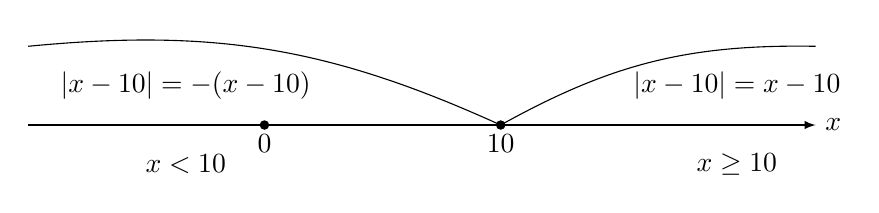
\begin{tikzpicture}[>=latex]
\draw[->](0,0)--(10,0)node [right]{$x$};
\foreach \x/\xtext in {3/0,6/10}
{
    \draw (\x, 0) [fill=black] circle (1.5pt)node[below]{$\xtext$}; 
}    
\draw (0,1) to [bend left=15] (6,0);
\draw (10,1) to [bend left=-15] (6,0);
\node at (2,.5){$|x-10|=-(x-10)$};
\node at (9,.5){$|x-10|=x-10$};
\node at (2,-.5){$x<10$};
\node at (9,-.5){$x\ge 10$};

\end{tikzpicture}
    \caption{}
\end{figure}

从而得到不等式$|x-10|\le 0.05$的解集:
\[\begin{split}
  &\quad   \{x|\; |x-10|\le 0.05\}\\
  &=\left\{x\Big| \begin{cases}
    -(x-10)\le 0.05\\x<10
\end{cases}\right\}\bigcup \left\{x\Big| \begin{cases}
    x-10\le 0.05\\x\ge 10
\end{cases}\right\}\\
&=\Big[\{x|-(x-10)\le 0.05\}\cap\{x|x<10\}\Big]\bigcup\Big[\{x|x-10\le 0.05\}\cap\{x|x\ge 10\}\Big]\\
&=\{x|9.95\le x<10\}\cup\{x|10\le x\le 10.05\}\\
&=\{x|9.95\le x\le 10.05\}
\end{split}
    \]

    同理可解例2.28:$|x+4|>9$,在这里零点是$x=-4$, 它把数轴分成两段:
    \begin{itemize}
        \item  当$x\ge -4$时,$|x+4|=x+4$;
        \item  当$x<-4$时,$|x+4|=-(x+4)$.
    \end{itemize}
    于是不等式的解集为:
\[\begin{split}
    &\quad \{x|\; |x+4|>9\} \\
&= \left\{x\Big|\begin{cases}
    -(x+4)>9\\x<-4
\end{cases}\right\}\bigcup \left\{x\Big|\begin{cases}
    x+4>9\\x\ge -4
\end{cases}\right\}\\
    &=\Big[\{x|-(x+4)>9\}\cap\{x|x<-4\}\Big]\bigcup\Big[\{x|x+4>9\}\cap\{x|x\ge -4\}\Big]\\
    &=\{x|x<-13\}\cup\{x|x>5\}
\end{split}\]

当然这种方法对解含一个绝对值的不等式不如前法方
便、但它具有一般性,且它可推广到解含二个、三个……绝
对值的不等式.

\begin{example}
    解不等式$|x-2|+|x+3|>7$.
\end{example}

\begin{solution}
这里$|x-2|$的零点为2; $|x+3|$的零点为$-3$,
把所有零点在数轴上按由小到大的次序排列,这样把数轴分
为下面的三段,而各段上的点和零点2的距离与该点和零
点$-3$的距离的和在脱去绝对值后的情况如图3.12所示.
\begin{figure}[htp]
    \centering
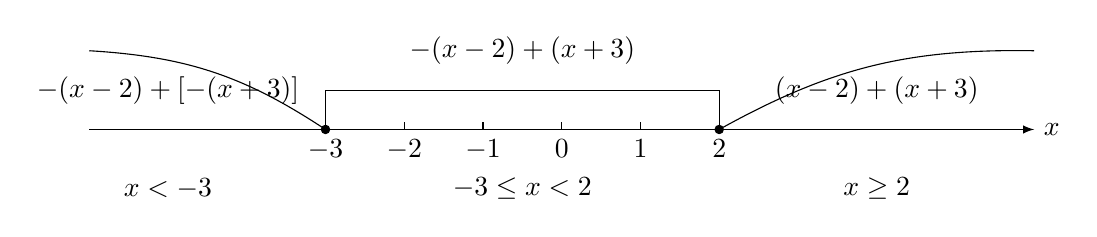
\begin{tikzpicture}[>=latex]
\draw[->] (-6,0)--(6,0)node[right]{$x$};
\foreach \x in {-3,-2,...,2}
{
    \draw (\x,0)node[below]{$\x$}--(\x,.1);
}
\draw (-3,0) [fill=black] circle(1.5pt);
\draw (2,0) [fill=black]circle (1.5pt);

\draw (-3,0)--(-3,.5)--(2,.5)--(2,0);
\draw (-6,1)to [bend left=15] (-3,0);
\draw (6,1)to [bend left=-15] (2,0);

\node at (-5,-.75){$x<-3$}; 
\node at (-.5,-.75){$-3\le x<2$};
\node at (4,-.75){$x\ge 2$};

\node at (-5,.5){$-(x-2)+[-(x+3)]$}; 
\node at (-.5,1){$-(x-2)+(x+3)$};
\node at (4,.5){$(x-2)+(x+3)$};
\end{tikzpicture}
\caption{}
\end{figure}

所以原不等式的解就是这三个解集的并集,即
\[\begin{split}
&\quad \left\{x\Big|\begin{cases}
    -(x-2)+[-(x+3)]>7\\
    x<-3
\end{cases}\right\}\bigcup \left\{x\Big|\begin{cases}
    -(x-2)+(x+3)>7\\ -3\le x<2
\end{cases}\right\}\\
&\qquad \bigcup \left\{x\Big|\begin{cases}
    (x-2)+(x+3)>7\\ x\ge 2
\end{cases}\right\}\\
&=\{x|x<-4\}\cup\emptyset \cup\{x|x>3\}\\
&=\{x|x<-4\}\cup \{x|x>3\}
\end{split}\]

\begin{figure}[htp]
    \centering
\begin{tikzpicture}[>=latex]
\draw[->](-6,0)--(5.5,0)node[right]{$x$};
\foreach \x in {-4,-3,...,3}
{
    \draw(\x,0)node[below]{$\x$}--(\x,.1);
}
\draw (-4,0)--(-4,.5)--(-6,.5);
\draw (3,0)--(3,.5)--(5,.5);
\fill[pattern=north east lines](-6,.5) rectangle (-4,0);
\fill[pattern=north east lines](5,.5) rectangle (3,0);
\draw (-4,0) [fill=white] circle (1.5pt);
\draw (3,0) [fill=white] circle (1.5pt);
\end{tikzpicture}
    \caption{}
\end{figure}
\end{solution}
    
\begin{ex}
\begin{enumerate}
    \item 解下列不等式:
\begin{multicols}{2}
\begin{enumerate}
    \item $|x-2|<5$
    \item $|2x-3|\ge 1$
    \item $|2-3x|\le 3$
    \item $|4x-5|<15$
    \item $\left|\frac{1}{2}x+1\right|<4$
    \item $|2x+5|<\frac{5}{12}$
    \item $\left|\frac{1}{2}x-4\right|+3>|8-x|$
    \item $|x|>2x-1$
\end{enumerate}    
\end{multicols}

\item 解下列不等式:
\begin{multicols}{2}
\begin{enumerate}
    \item $|x+1|+|x-1|>0$
    \item $|x+3|-|x-3|<5$
    \item $|x-5|-|x+3|>3$
    \item $|x-1|-11<2$
\end{enumerate}
\end{multicols}
\item 用宽6cm的铁板,截一个面积为48${\rm cm}^2$的长方形零件,
要求面积的绝对误差不超过0.3${\rm cm}^2$, 长度应在什么范围
内?
\item 解下列不等式:
\begin{enumerate}
    \item $3|x-6|+|x+2|-|x-0.5|\le 7$
    \item $|x|+|x-1|+|x-2|\ge 4$
\end{enumerate}
\end{enumerate}
\end{ex}

\subsection{一元二次不等式}
形如
\[ax^2+bx+c>0 \qquad \text{或}\qquad  ax^2+bx+c<0 \]
的不等式称为一元二次不等式.这里$a\ne 0$.

我们首先说明下面的定理:
\begin{blk}{定理1}
    设$b^2-4ac\le 0$, 则
\begin{enumerate}
    \item 当$a>0$时,不论$x$为何值,$ax^2+bx+c\ge 0$
    \item 当$a<0$时,不论$x$为何值,$ax^2+bx+c\le 0$
\end{enumerate} 
上面两个不等式仅在$b^2-4ac=0$, 且
$x=-\frac{b}{2a}$时等式成立.
\end{blk}

这个定理的证明已在本章的例3.12中用配方法证过了.
建议读者再复习一遍它的证明.

这个定理告诉我们;不管$b^2-4ac<0$还是$b^2-4ac=0$,
二次三项式$ax^2+bx+c$的值除可能是0外,符号总是和二次
项的系数$a$的符号一致,不随$x$的改变而改变的.

根据这个结论,我们知道不等式:
\begin{enumerate}
    \item $ax^2+bx+c>0$ $(a>0,\; b^2-4ac<0)$的解集
    是:$\{x|x\in\mathbb{R}\}$.
    \item $ax^2+bx+c>0$ $(a>0,\;b^2-4ac=0)$的解集是:
    $\left\{x\Big|x\in\mathbb{R},\; x\ne -\frac{b}{2a}\right\}$
    \item $ax^2+bx+c<0$ $(a>0,\; b^2-4ac<0)$的解集是
    空集$\emptyset$.
\end{enumerate}

但当$b^2-4ac>0$时,$ax^2+bx+c$的值的情形是怎样的
呢?这时$ax^2+bx+c$的值的符号要因$x$的值不同而改变,现在
我们就来讨论它的值的符号怎样随$x$的取值改变.

当$b^2-4ac>0$. 而$a\ne 0$时,$ax^2+bx+c=0$有两个不同
的实根$x_1$和$x_2$, 并设$x_1<x_2$, 于是根据因式定理有:
\[ax^2+bx+c=a(x-x_1)(x-x_2)\]

在这里,我们只要记住一个最简单的原则,就可以解决
问题,那就是“奇数个负数相乘是负的,偶数个负数相乘是
正的”,例如当$x_1<x<x_2$时,$x-x_1$是正的而$x-x_2$是负的,于是
$(x-x_1)(x-x_2)<0$, 因此在这时$ax^2+bx+c$的值的符号与$a$
相反,从此我们可以把结果列成一个表.
\begin{center}
\begin{tabular}{c|c|c}
\hline
      & $x<x_1$ & $ax^2+bx+c>0$\\
 $a>0$   &  $x_1<x<x_2$ & $ax^2+bx+c<0$\\
    &  $x_2<x$ & $ax^2+bx+c>0$\\
\hline
  & $x<x_1$ & $ax^2+bx+c<0$\\
$a<0$&  $x_1<x<x_2$ & $ax^2+bx+c>0$\\
&  $x_2<x$ & $ax^2+bx+c<0$\\
\hline
\end{tabular}
\end{center}

我们把上面讨论的结果总结成下面的定理:
\begin{blk}{定理2}
    设$b^2-4ac>0$, 则当$x$的取值在$ax^2+bx+c$的
    二根之间时,$ax^2+bx+c$的值的符号与$a$的符号相反;当$x$的
    取值在二根之间的以外部分时,$ax^2+bx+c$的值的符号与$a$
    的符号相同. 
\end{blk}

\begin{center}
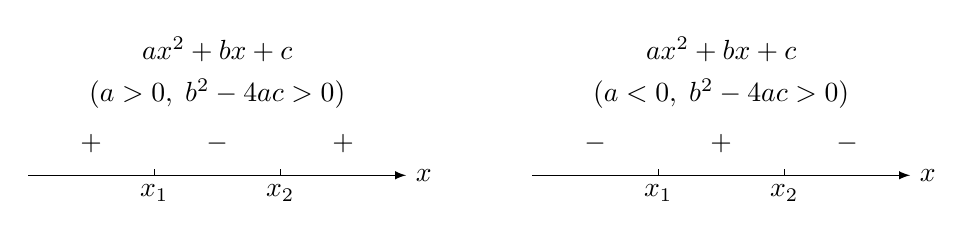
\begin{tikzpicture}[>=latex, scale=.8]
\begin{scope}
\draw[->] (0,0)--(6,0)node[right]{$x$};
\foreach \x/\xtext in {2/x_1,4/x_2}
{
    \draw (\x,0)node[below]{$\xtext$}--(\x,.1);
}
\foreach \x/\xtext in {1/+,3/-,5/+}
{
    \node at (\x,.5){$\xtext$};
}
\node at (3,2){$ax^2+bx+c$};
\node at (3,1.3){$(a>0,\; b^2-4ac>0)$};
\end{scope}
\begin{scope}[xshift=8cm]
\draw[->] (0,0)--(6,0)node[right]{$x$};
\foreach \x/\xtext in {2/x_1,4/x_2}
{
    \draw (\x,0)node[below]{$\xtext$}--(\x,.1);
}
\foreach \x/\xtext in {1/-,3/+,5/-}
{
    \node at (\x,.5){$\xtext$};
}
\node at (3,2){$ax^2+bx+c$};
\node at (3,1.3){$(a<0,\; b^2-4ac>0)$};
\end{scope}
\end{tikzpicture} 
\end{center}

再把定理1和定理2的结论综合起来看,我们说:$ax^2+
bx+c\; (a\ne 0)$的值的符号和它的二次项的系数的符号相同,
除非$x$的值是在它的二根之间或等于它的根.



\begin{example}
 解不等式$-x^2+2x-2>0$
\end{example}

\begin{solution}
 由于$a=-1<0$, 且$b^2-4ac=2^2-4(-1)\cdot(-2)=-4<0$, $-x^2+2x-2$的值对于任何$x$都是负的,
故不等式无解.   
\end{solution}

\begin{example}
   解不等式$2x^2-4x+3>0$ 
\end{example}

\begin{solution}
    由于$a=2>0$, 且$b^2-4ac=(-4)2-4\cdot 2\cdot 3=-8<0$, 故不等式的解集是一切实数.
\end{solution}

\begin{example}
 解不等式$2x^2-4x-5\le 0$   
\end{example}

\begin{solution}
    由于$b^2-4ac=(-4)2-4\x2\x(-5)=56>0$,
所以对应的二次方程有两个实根:
\[x_1=\frac{2-\sqrt{14}}{2},\qquad x_2=\frac{2+\sqrt{14}}{2}\]
又$a=2>0$, 所以要使原不等式成立,它的解必须且只须在
二根之间,或等于二根.因此解集为:
\[\left\{x\Big|\frac{2-\sqrt{14}}{2}\le x\le \frac{2+\sqrt{14}}{2} \right\}\]
\end{solution}

\begin{example}
解不等式$4x^2-12x+9\le 0$
\end{example}

\begin{solution}
    由于$b^2-4ac=(-12)^2-4\x4\x9=0$, 故
\[4x^2-12x+9=(2x-3)^2\]
因此解集只能是$\left\{\frac{3}{2}\right\}$.
\end{solution}


\begin{example}
    $p$为何值时,二次三项式
$x^2+(p-2)x+2p+1$
对于任何$x$都取正值.
\end{example}


\begin{solution}
    只有当判别式$\Delta<0$时,$x^2+(p-2)x+2p+1$
的值才能保持正号,因此
$$\Delta=(p-2)2-4(2p+1)<0$$
即$p(p-12)<0$.

解$p(p-12)=0$, 得到二根$p_1=0$, $p_2=12$, 又$p^2$的系数是
$1>0$, 因此上面不等式的解满足$0<p<12$.

答:在$0<p<12$的条件下,$x^2+(p-2)x+2p+1$
对于任何$x$值都取正值.
\end{solution}


\begin{ex}
\begin{enumerate}
    \item 解下列不等式:
\begin{multicols}{2}
\begin{enumerate}
    \item $(x-2)^2+1>0$
    \item $(x-2)^2-1>0$
    \item $x^2-x+\frac{1}{4}>0$
    \item $2x^2-3x>2$
    \item $x^2>0$
    \item $x^2-4x+6\le 0$
    \item $49x^2+168x+144\le 0$
    \item $x^2+x+\frac{1}{4}\le 0$
    \item $x^2+x+2>0$
    \item $x^2+x-2<0$
\end{enumerate}
\end{multicols}
    \item $m$为何值使得下面的二次三项式的值对于任何$x$值都是
    正的或都是负的:
\begin{multicols}{2}
\begin{enumerate}
    \item $x^2-8x+m+10$
    \item $-x^2-2x+m-6$
    \item $x^2+(m+2)x+3m+1$
    \item $-3x^2+(2m+6)x-m-3$
\end{enumerate}
\end{multicols}
\end{enumerate}    
\end{ex}

\subsection{一元高次不等式}
如果一元较高次多项式能分解成一次或二次的因式的乘
积,上节所述对一元二次不等式的解法的原则,也可以用来
解较高次不等式.

现在我们把上节对解二次不等式所采用的原则概括成以
下的步骤:
\begin{enumerate}
    \item 把不等式化成标准型:$p(x)>0$或$p(x)<0$. 这里
$p(x)$是个一元多项式.
\item 把$p(x)$因式分解
\item 求出各个因式的零点.
\item 把零点在数轴上由小到大排列起来,并把数轴分为
若干段.
\item 在各段上考察各个因式的符号并决定$p(x)$的符号.
\item 找出不等式的解集.
\end{enumerate}


\begin{example}
    解不等式:$x^3+3x^2>2x+6$
\end{example}

\begin{solution}
\begin{enumerate}
    \item 把原不等式化为如下的标准型:$x^3+3x^2-2x-6>0$
    \item 把不等式左端因式分解:
    \[\begin{split}
         x^3+3x^2-2(x+3)&=x^2(x+3)-2(x+3)\\
    &=(x+3)(x^2-2)\\
    &=(x+3)\left(x+\sqrt{2}\right)\left(x-\sqrt{2}\right) 
    \end{split}\]
  
    所以解原不等式,就相当于解不等式
   \[(x+3)\left(x+\sqrt{2}\right)\left(x-\sqrt{2}\right) >0\]
    \item 各个因子的零点是$-3,-\sqrt{2},\sqrt{2}$.
    
    4, 5, 6三步可列表进行:
\begin{center}
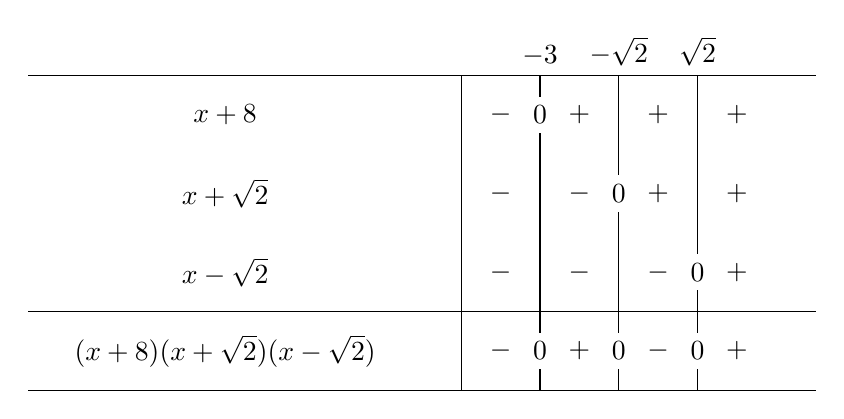
\begin{tikzpicture}[yscale=2]
\foreach \x in {0,.5,2}
{
    \draw (0,\x)--(10,\x);
}
\foreach \x/\xtext in {5.5/{},6.5/-3,7.5/-\sqrt{2},8.5/\sqrt{2}}
{
    \draw (\x,0)--(\x,2)node[above]{$\xtext$};
}

\node at (2.5,.25){$(x+8)(x+\sqrt{2})(x-\sqrt{2})$};
\foreach \x/\xtext in {6/-,7/+,8/-,9/+}
{
    \node at (\x,.25) {$\xtext$};
}

\node at (2.5,.75){$x-\sqrt{2}$};
\foreach \x/\xtext in {6/-,7/-,8/-,9/+}
{
    \node at (\x,.75) {$\xtext$};
}

\node at (2.5,1.25){$x+\sqrt{2}$};
\foreach \x/\xtext in {6/-,7/-,8/+,9/+}
{
    \node at (\x,1.25) {$\xtext$};
}

\node at (2.5,1.75){$x+8$};
\foreach \x/\xtext in {6/-,7/+,8/+,9/+}
{
    \node at (\x,1.75) {$\xtext$};
}


\node at (6.5,1.75)[fill=white] {0};
\node at (6.5,.25)[fill=white] {0};
\node at (7.5,.25)[fill=white] {0};
\node at (8.5,.25)[fill=white] {0};
\node at (8.5,.75)[fill=white] {0};
\node at (7.5,1.25)[fill=white] {0};
\end{tikzpicture}
\end{center}
\end{enumerate}

所以原不等式的解集为:
\[\{x|-3<x<-\sqrt{2}\}\cup\{x|x>\sqrt{2}\}\]
\end{solution}

\begin{example}
解不等式$(x^2-3)(x^2-5)\le 0$
\end{example}


\begin{solution}
    解原不等式就相当于解不等式
\[(x+\sqrt{3})(x-\sqrt{3})(x+\sqrt{5})(x-\sqrt{5})\le 0\]
列表解之如下:
\begin{center}
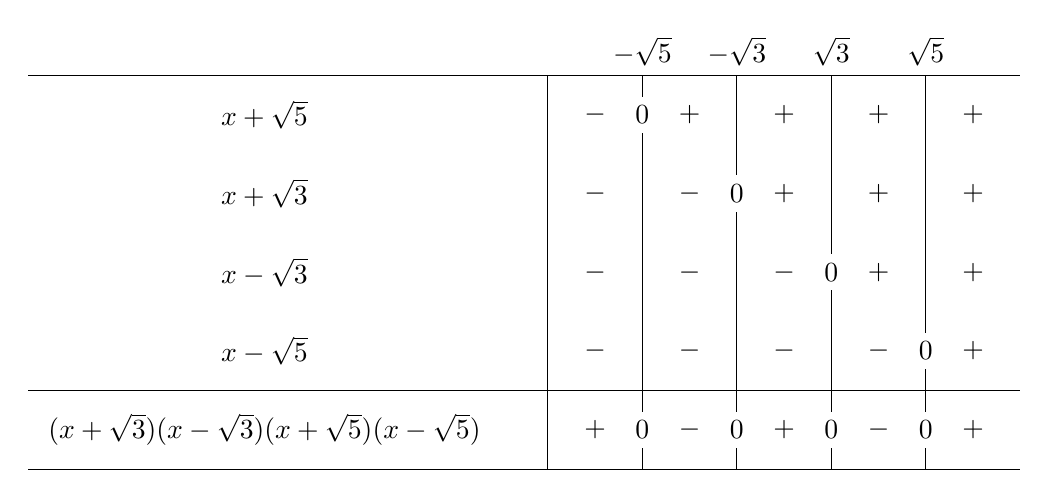
\begin{tikzpicture}[yscale=2, xscale=1.2]
\foreach \x in {0,.5,2.5}
{
    \draw (0,\x)--(10.5,\x);
}
\foreach \x/\xtext in {5.5/{},6.5/-\sqrt{5},7.5/-\sqrt{3},8.5/\sqrt{3},9.5/\sqrt{5}}
{
    \draw (\x,0)--(\x,2.5)node[above]{$\xtext$};
}

\node at (2.5,.25){$(x+\sqrt{3})(x-\sqrt{3})(x+\sqrt{5})(x-\sqrt{5})$};
\foreach \x/\xtext in {6/+,7/-,8/+,9/-,10/+}
{
    \node at (\x,.25) {$\xtext$};
}

\node at (2.5,.75){$x-\sqrt{5}$};
\foreach \x/\xtext in {6/-,7/-,8/-,9/-,10/+}
{
    \node at (\x,.75) {$\xtext$};
}

\node at (2.5,1.25){$x-\sqrt{3}$};
\foreach \x/\xtext in {6/-,7/-,8/-,9/+,10/+}
{
    \node at (\x,1.25) {$\xtext$};
}

\node at (2.5,1.75){$x+\sqrt{3}$};
\foreach \x/\xtext in {6/-,7/-,8/+,9/+,10/+}
{
    \node at (\x,1.75) {$\xtext$};
}

\node at (2.5,2.25){$x+\sqrt{5}$};
\foreach \x/\xtext in {6/-,7/+,8/+,9/+,10/+}
{
    \node at (\x,2.25) {$\xtext$};
}

\foreach \x in {6.5,7.5,8.5,9.5}
{
    \node at (\x,.25)[fill=white] {0};
}
\node at (9.5,.75)[fill=white] {0};
\node at (7.5,1.75)[fill=white] {0};
\node at (6.5,2.25)[fill=white] {0};
\node at (8.5,1.25)[fill=white] {0};
\end{tikzpicture}
\end{center}

所以原不等式的解集为:
\[\{x|-\sqrt{5}\le x\le -\sqrt{3}\}\cup\{x|\sqrt{3}\le x\le \sqrt{5}\}\]
\end{solution}

\begin{example}
    解不等式$(x^3-1)(x^3+2x^2-x-2)>0$
\end{example}

\begin{solution}
    将不等式左侧因式分解后就相当于解不等式:
$$(x-1)^2(x^2+x+1)(x+1)(x+2)>0$$
这里二次三项式$x^2+x+1$的判别式小于零,且首项系数大
于零,故它对一切实数值都大于零,因此在列表时可以把它
略去不计.但因子$(x-1)^2$, 除$x=1$的零点外,$(x-1)^2$恒
大于零,故也可暂不考虑它,不过在最后确定解集时,要把
$x=1$除外的情况考虑进去.这样,就有下表:
\begin{center}
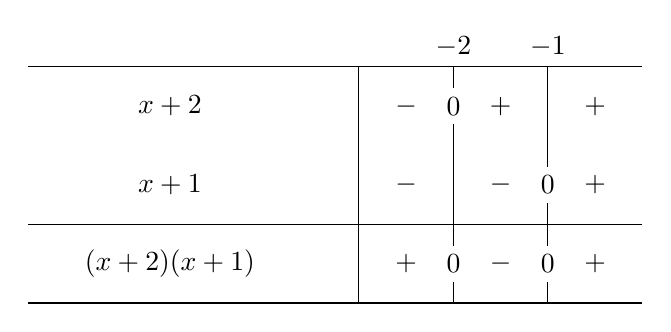
\begin{tikzpicture}[yscale=2, xscale=1.2]
\foreach \x in {0,.5,1.5}
{
    \draw (2,\x)--(8.5,\x);
}
\foreach \x/\xtext in {5.5/{},6.5/-2,7.5/-1}
{
    \draw (\x,0)--(\x,1.5)node[above]{$\xtext$};
}

\node at (3.5,.25){$(x+2)(x+1)$};
\foreach \x/\xtext in {6/+,7/-,8/+}
{
    \node at (\x,.25) {$\xtext$};
}

\node at (3.5,.75){$x+1$};
\foreach \x/\xtext in {6/-,7/-,8/+}
{
    \node at (\x,.75) {$\xtext$};
}

\node at (3.5,1.25){$x+2$};
\foreach \x/\xtext in {6/-,7/+,8/+}
{
    \node at (\x,1.25) {$\xtext$};
}

\node at (6.5,.25)[fill=white] {0};
\node at (7.5,.25)[fill=white] {0};
\node at (7.5,.75)[fill=white] {0};
\node at (6.5,1.25)[fill=white] {0};
\end{tikzpicture}
\end{center}

考虑$(x-1)^2(x^2+x+1)(x+1)(x+2)>0$
的解时,要把$x=1$除外,故解集为:
\[\{x|x<-2\}\cup\{x|x>-1,\; x\ne 1\}\]
或者写成
\[\{x|x<-2\}\cup \{x|-1<x<1\}\cup\{x|x>1\}\]
\end{solution}

\begin{example}
    解不等式$\frac{9-x^2}{x^2-x-2}\ge 0$
\end{example}

\begin{solution}
解法1:用化为不等式组的方法解
\[\begin{split}
&\quad \left\{x\Big| \frac{9-x^2}{x^2-x-2}\ge 0\right\}\\
&=\left\{x\Big|\begin{cases}
    9-x^2\ge 0\\ x^2-x-2>0
\end{cases} \right\}\bigcup \left\{x\Big|\begin{cases}
    9-x^2\le 0\\ x^2-x-2<0
\end{cases} \right\}\\
&=\Big[\{x|-3\le x\le 3\}\cap \{x|x<-1\text{ 或 }x>2\}\Big]\\
&\qquad \bigcup \Big[\{x|x\le-3\text{ 或 }x\ge 3\}\cap \{x|-1<x<2\}\Big]\\
&=\Big[\{x|-3\le x<-1\}\cup\{x|2<x\le 3\} \Big]\cup \big[\emptyset\cup\emptyset\big]\\
&=\{x|-3\le x<-1\}\cup\{x|2<x\le 3\}
\end{split}\]

解法2: 用列表法来解.

事实上,解原不等式就相当于解不等式组
\[\begin{cases}
    (x+3)(x+1)(x-2)(x-3)\le 0\\
    x\ne -1,\quad x\ne 2
\end{cases}\]

\begin{center}
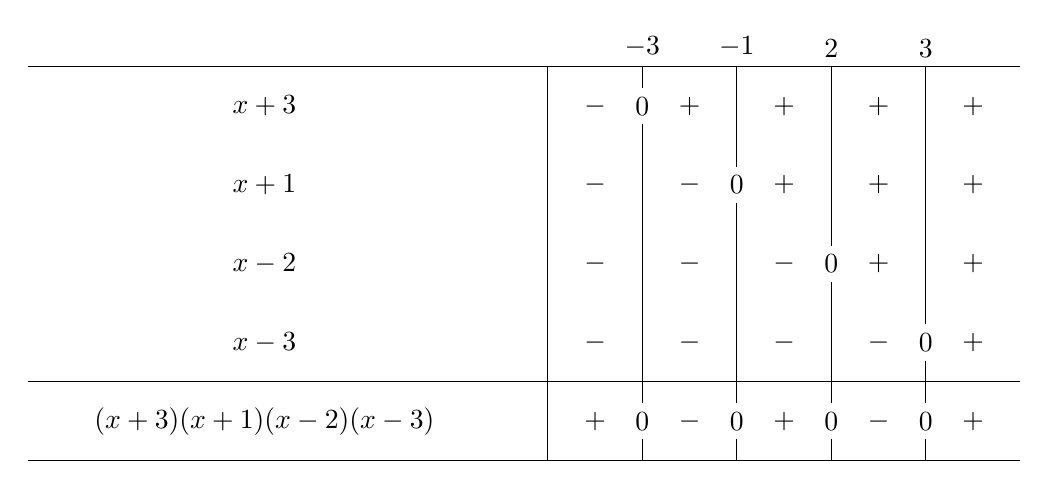
\begin{tikzpicture}[yscale=2, xscale=1.2]
\foreach \x in {0,.5,2.5}
{
    \draw (0,\x)--(10.5,\x);
}
\foreach \x/\xtext in {5.5/{},6.5/-3,7.5/-1,8.5/2,9.5/3}
{
    \draw (\x,0)--(\x,2.5)node[above]{$\xtext$};
}

\node at (2.5,.25){$(x+3)(x+1)(x-2)(x-3)$};
\foreach \x/\xtext in {6/+,7/-,8/+,9/-,10/+}
{
    \node at (\x,.25) {$\xtext$};
}

\node at (2.5,.75){$x-3$};
\foreach \x/\xtext in {6/-,7/-,8/-,9/-,10/+}
{
    \node at (\x,.75) {$\xtext$};
}

\node at (2.5,1.25){$x-2$};
\foreach \x/\xtext in {6/-,7/-,8/-,9/+,10/+}
{
    \node at (\x,1.25) {$\xtext$};
}

\node at (2.5,1.75){$x+1$};
\foreach \x/\xtext in {6/-,7/-,8/+,9/+,10/+}
{
    \node at (\x,1.75) {$\xtext$};
}

\node at (2.5,2.25){$x+3$};
\foreach \x/\xtext in {6/-,7/+,8/+,9/+,10/+}
{
    \node at (\x,2.25) {$\xtext$};
}

\foreach \x in {6.5,7.5,8.5,9.5}
{
    \node at (\x,.25)[fill=white] {0};
}
\node at (9.5,.75)[fill=white] {0};
\node at (7.5,1.75)[fill=white] {0};
\node at (6.5,2.25)[fill=white] {0};
\node at (8.5,1.25)[fill=white] {0};
\end{tikzpicture}
\end{center}

考虑原不等式的解,要把$x=-1$和$x=2$除外,所以原
不等式的解集
\[\{x|-3\le x<-1\}\cup \{2<x\le 3\}\]
\end{solution}



\begin{ex}
 \begin{enumerate}
     \item 解下列不等式:
\begin{enumerate}
    \item $(x-2)(x+3)(x-4)(x+5)>0$
    \item $x^2(x+11)\ge 6(x^2+1)+x-1$
    \item $(x-2)(3x^2+2x-5)<0$
    \item $x^3+7x^2+6x\le 0$
\end{enumerate}
     \item      解下列不等式:
    \begin{multicols}{2}
\begin{enumerate}
    \item $\frac{2x-7}{x-5}>0$
    \item $\frac{(3x+2)(2x+3)}{(3x-2)(2x-3)}\ge 0$
    \item $\frac{x^2+2x-3}{x^2-2x-8}\le 0$
    \item $\frac{x+1}{x-1}<\frac{x-9}{x-3}-2$
\end{enumerate}        
    \end{multicols}
 \end{enumerate}   
\end{ex}

\section*{复习题三}
\addcontentsline{toc}{section}{复习题三}
\begin{enumerate}
\item   设$a,b,m$都是正数,如果$a<b$, 则
$\frac{a+m}{b+m}>\frac{a}{b}$;
如果$a>b$,则$\frac{a+m}{b+m}<\frac{a}{b}$
试证之.

\item  已知$a\ne b$, 求证:
\begin{multicols}{2}
\begin{enumerate}
    \item $a^2+3b^2>2b(a+b)$
    \item $a^4+6a^2b^2+b^4>4ab(a^2 +b^2)$
    \item $(a-b)(a+b)>-2b^2$
    \item $a^4+b^4>a^3b+ab^3$
\end{enumerate}
\end{multicols}

\item 已知$a$、$b$、$c$是不相等的正数,求证:
\begin{enumerate}
    \item $(a+b)(b+c)(c+a)>8abc$
    \item $\frac{b+c-a}{a}+\frac{c+a-b}{b}+\frac{a+b-c}{c}>3$
    \item $(ab+a+b+1)(ab+ac+bc+c^2)>16abc$
\end{enumerate}

\item 已知$a^2+b^2=1$, $x^2+y^2=1$, 求证:$ax+by\le 1$.
\item 若$x,y,z$是正数,且$x+y+z=1$,求证:
$x^2+y^2+z^2\ge \frac{1}{3}$.
\item \begin{enumerate}
    \item 试证:两正数之和与此两正数的倒数之和的乘积不小于4.
    \item 试证:$\frac{\lg^2x+2}{\sqrt{\lg^2x+1}}\ge 2$.
\end{enumerate}
\item 已知$\triangle ABC$的三边为$a$、$b$、$c$且
\[c=\frac{a^2+3}{4},\qquad b=\frac{a^2-2a-3}{4}\]
求证$c$边最大.
\item 
已知直角三角形斜边为定值,求这个直角三角形面积的
最大值,并指出取得最大值的条件.
\item 
解下列关于$x$的不等式:
\begin{multicols}{2}
\begin{enumerate}
    \item $ax+b^2>bx+a^3\quad (a<b)$
    \item $mx-n^3<nx-m^3\quad (m<n)$
    \item $ax+b>cx+d$
    \item $\frac{2x}{2-h}-\frac{h(x+1)}{2-h}<1\quad (h\ne 2)$
    \item $\frac{x-a}{x-b}>0$
\end{enumerate}
\end{multicols}
\item 解不等式组:
\begin{enumerate}
    \item $\begin{cases}
        (x-1)^2<(x+1)^3-4\\(x-1)(x-2)<(x+3)(x-4)+20
    \end{cases}$
    \item $\begin{cases}
        (x+2)^3-(x-1)^3<9x^2 \\(x+2)^2-(x-1)^2>9
    \end{cases}$
\end{enumerate}

\item 求下列不等式组的整数解:
\begin{multicols}{2}
\begin{enumerate}
    \item $\begin{cases}
        2x-7>0\\3x-5<15
    \end{cases}$
    \item $\begin{cases}
        11x-5<13\\3x+2>-5
    \end{cases}$
    \item $\begin{cases}
       3x+10>0\\ \frac{15}{3}x-10<4x
    \end{cases}$
    \item $\begin{cases}
      \frac{2x-11}{4}+\frac{19-2x}{2}>-2x\\
      \frac{2x+15}{9}>\frac{1}{5}(x-1)+\frac{x}{3}
    \end{cases}$
\end{enumerate}
\end{multicols}

\item 解下列不等式,并在数轴上把解集表示出来:
\begin{multicols}{2}
\begin{enumerate}
    \item $|x+2|-|x-3|<4$
    \item $|x-5|-|x-4|\ge 3$
    \item $|x-2|\ge 2x-1$
    \item $|2x^2+5x-2|<1$
\end{enumerate}
\end{multicols}

\item 一个两位数,它的个位数字比十位数字大2, 已知这个
两位数小于45而大于24, 求这数.

\item 一个两位数,它大于22而小于36, 并且它的十位数字比
个位数字大3, 求这数.
\item 一个分数的分子、分母都是自然数,分子比分母小1,
如果分子,分母都加上1, 所得就大于$\frac{1}{2}$,如果分子,
分母都减去1所得就小于$\frac{6}{7}$, 求这个分数.
\item 当$m$是什么实数时,方程
$mx^2-(m+1)x+3=0$
有实数根?没有实数根.
\item $a$是什么实数时,方程$5x-2a=ax-4-x$的解在2和
10之间?
\item $t$是什么实数时,方程
$tx^2-(1-t)x+t=0$
没有实数解?
\item 讨论二次三项式$x^2+2x+m+1$的值的符号.
\item 造一个截面为矩形的水管,要求矩形的长比宽多10cm, 
并且面积不小于250${\rm cm}^2$, 矩形的宽至少应当是多少cm?
\item 要使下列各式有意义,$x$的值应有什么限制?
\begin{enumerate}
    \item $\frac{\sqrt{x-3}}{\sqrt{x^2-3x+2}}$
    \item $\sqrt{|x-2|-3}+\frac{1}{\sqrt[3]{2x+1}}$
\end{enumerate}
\item $m$为何值使得下列不等式对于$x$的一切值都成立:
\begin{enumerate}
    \item $mx^2+12x-5<0$
    \item $(m+3)x^2-5x-4<0$
    \item $(m-2)x^2-2(2m-3)x+5m-6>0$
    \item $(m^2+6m-4)x^2-2(m-1)x+2<0$
    \item $(m^2+4m-5)x^2-2(m+1)x+3>0$
\end{enumerate}

\item 解下列不等式:
\begin{multicols}{2}
\begin{enumerate}
    \item $\frac{(x-1)(x-2)}{x-3}\ge 0$
    \item $\frac{x^2-6x+18}{x-4}<0$
    \item $\frac{x^2+2x-3}{x^2-2x+8}>0$
    \item $\frac{x^2+5x+4}{x^2-5x-6}<0$
    \item $2-\frac{x-3}{x-2}>\frac{x-2}{x-1}$
    \item $3-\frac{2x-17}{x-5}>\frac{x-5}{x+2}$
\end{enumerate}
\end{multicols}

\end{enumerate}







